\documentclass[11pt,a4paper]{report}
\usepackage{fontspec}
\usepackage[french]{babel}
\setmainfont{Calibri}
\setmonofont{Consolas}[Scale=0.92]
\usepackage[a4paper,top=2.2cm,bottom=2.2cm,left=2.4cm,right=2.4cm]{geometry}
\usepackage{xcolor}
\definecolor{emerald}{RGB}{14,124,102}
\definecolor{emeraldDark}{RGB}{10,92,76}
\definecolor{hdr}{RGB}{220,240,234}
\definecolor{codeBg}{RGB}{242,242,242}
\usepackage{graphicx}
\usepackage{array}
\usepackage{colortbl}
\usepackage{tabularx}
\usepackage{caption}
\captionsetup{font=small,labelfont=bf,labelsep=period,justification=centering}
\usepackage{titlesec}
\titleformat{\chapter}[block]
  {\normalfont\LARGE\bfseries\color{emeraldDark}}{}{0pt}{}
  [\vspace{2pt}{\color{emerald}\rule{\textwidth}{1pt}}]
\titlespacing*{\chapter}{0pt}{24pt}{18pt}
\titleformat{\section}
  {\normalfont\Large\bfseries\color{emerald}}{}{0pt}{}
\titleformat{\subsection}
  {\normalfont\large\bfseries\color{black!70}}{}{0pt}{}
\usepackage{fancyhdr}
\pagestyle{fancy}
\fancyhf{}
\fancyfoot[C]{\small\thepage}
\renewcommand{\headrulewidth}{0pt}
\fancypagestyle{plain}{\fancyhf{}\fancyfoot[C]{\small\thepage}\renewcommand{\headrulewidth}{0pt}}
\usepackage{listings}
\lstset{
  basicstyle=\ttfamily\footnotesize\color{black!85},
  backgroundcolor=\color{codeBg},
  frame=single, rulecolor=\color{gray!55},
  breaklines=false, columns=fullflexible, keepspaces=true,
  aboveskip=10pt, belowskip=10pt, xleftmargin=6pt, xrightmargin=6pt,
  showstringspaces=false
}
\usepackage{hyperref}
\hypersetup{colorlinks=true, linkcolor=emeraldDark, urlcolor=emerald, pdftitle={Rapport de stage MaintenX}, pdfauthor={Othmane LAADIOUI}}
\setlength{\parskip}{4pt}
\begin{document}
\begin{titlepage}
\thispagestyle{empty}
\noindent\colorbox{emerald}{\parbox{\dimexpr\textwidth-2\fboxsep\relax}{\centering\bfseries\color{white}\fontsize{13}{16}\selectfont ROYAUME DU MAROC\\[2pt] École Marocaine des Sciences de l'Ingénieur (EMSI)}}
\vspace{2.4em}
\begin{center}
{\bfseries\color{emeraldDark}\large Département : Ingénierie Informatique et Réseaux (IIR)}\\[2pt]
3ème année — Cycle Ingénieur
\vspace{2.5em}

\begin{tabular}{@{}c@{\hspace{2.5em}}c@{}}

\includegraphics[height=1.6cm]{../images/emsilogo.png} &

\includegraphics[height=1.6cm]{../images/logosirecom.png}
\end{tabular}
\vspace{3em}

{\LARGE\bfseries\color{emerald} RAPPORT DE STAGE}\\[4pt]
{\itshape Réalisé au sein de la société SIRECOM}
\vspace{3em}

{\huge\bfseries\color{emeraldDark} MAINTENX}\\[6pt]
{\large Application de gestion des interventions de maintenance}
\vspace{3em}

\begin{tabular}{>{\columncolor{hdr}\bfseries\color{emeraldDark}\raggedright\arraybackslash}p{4.5cm}>{\raggedright\arraybackslash}p{9.5cm}}
\hline
Réalisé par & M. Othmane LAADIOUI\\\hline
Encadrante académique & Mme Safaa FOUAD (EMSI)\\\hline
Encadrants de stage & M. Anass EL GHAZI (SIRECOM)\\\hline
Encadrant de stage & M. Youness DRISSI (SIRECOM)\\\hline
Période de stage & Six semaines\\\hline
\end{tabular}
\end{center}
\vfill
\noindent\colorbox{emerald}{\parbox{\dimexpr\textwidth-2\fboxsep\relax}{\centering\bfseries\color{white}\fontsize{12}{14}\selectfont Année universitaire 2025 - 2026 \quad|\quad Société : SIRECOM}}
\end{titlepage}
\phantomsection
\chapter*{Remerciements}
\addcontentsline{toc}{chapter}{Remerciements}

Avant tout développement, il m'est agréable d'exprimer ma profonde gratitude à toutes les personnes qui ont contribué, de près ou de loin, à la réussite de ce projet de fin d'études.

Je tiens tout d'abord à remercier \textbf{l'École Marocaine des Sciences de l'Ingénieur (EMSI)} pour la qualité de la formation qui m'a été dispensée et pour m'avoir offert l'opportunité d'effectuer un stage au sein d'une entreprise réputée dans le domaine des systèmes d'information.

Mes sincères remerciements vont à \textbf{Mme Safaa FOUAD}, mon encadrante académique, pour son encadrement pédagogique, ses conseils avisés, sa disponibilité et son suivi régulier tout au long de la réalisation de ce projet.

Je remercie chaleureusement \textbf{M. Anass EL GHAZI} et \textbf{M. Youness DRISSI}, mes encadrants au sein de la société \textbf{SIRECOM}, pour leur accueil, leur confiance, leur encadrement technique de qualité et pour toutes les connaissances professionnelles qu'ils m'ont transmises durant ces six semaines de stage.

Je remercie également l'ensemble du personnel de la société SIRECOM pour son accueil chaleureux et sa collaboration, ainsi que tous mes enseignants de l'EMSI qui ont contribué à ma formation.

Enfin, je dédie ce travail à ma famille et à mes proches pour leur soutien moral inconditionnel tout au long de mes études.
\phantomsection
\chapter*{Résumé}
\addcontentsline{toc}{chapter}{Résumé}

Dans le cadre de mon projet de fin d'études effectué au sein de la société \textbf{SIRECOM}, j'ai conçu et développé \textbf{MaintenX}, une application de bureau en \textbf{Java Swing} dédiée à la gestion des interventions de maintenance. Le projet répond à une problématique concrète : la gestion des demandes d'intervention était réalisée de manière manuelle (cahiers, tableurs Excel, échanges téléphoniques), ce qui engendrait des pertes d'information, une mauvaise priorisation des urgences, des affectations de techniciens peu efficaces et l'absence d'historique fiable.

MaintenX permet d'automatiser l'ensemble du cycle de vie d'une intervention de maintenance : création de la demande, affectation d'un technicien, suivi du statut (ouverte, affectée, en cours, en attente, terminée, annulée), enregistrement des diagnostics et des solutions, clôture avec coûts associés, recherche multicritère, tableau de bord statistique et journal d'activité. L'application repose sur une architecture multicouche \textbf{Vue $\rightarrow$ Contrôleur $\rightarrow$ Service $\rightarrow$ DAO $\rightarrow$ MySQL} qui garantit la séparation des responsabilités et la maintenabilité du code. Les mots de passe sont sécurisés par hachage \textbf{BCrypt} et chaque action sensible est tracée dans un historique.

Le résultat final est une application \textbf{complète, testée et documentée}, livrée sous forme d'un JAR exécutable avec un jeu de données de démonstration intégré pour faciliter la soutenance.

\textbf{Mots-clés :} gestion de maintenance, application de bureau, Java, Swing, JDBC, MySQL, architecture multicouche, UML, tests unitaires.
\phantomsection
\chapter*{Abstract}
\addcontentsline{toc}{chapter}{Abstract}

As part of my end-of-studies project carried out within \textbf{SIRECOM} company, I designed and developed \textbf{MaintenX}, a \textbf{Java Swing} desktop application dedicated to maintenance intervention management. The project addresses a concrete issue: intervention requests were handled manually (notebooks, Excel spreadsheets, phone calls), which led to information loss, poor prioritisation of urgent requests, inefficient technician assignment and the lack of a reliable history.

MaintenX automates the whole lifecycle of a maintenance intervention: request creation, technician assignment, status tracking (open, assigned, in progress, on hold, completed, cancelled), diagnostics and solutions recording, closure with related costs, multi-criteria search, statistics dashboard and activity log. The application relies on a multi-layered architecture \textbf{View $\rightarrow$ Controller $\rightarrow$ Service $\rightarrow$ DAO $\rightarrow$ MySQL} which guarantees separation of concerns and code maintainability. Passwords are secured with \textbf{BCrypt} hashing and every sensitive action is traced in a history log.

The final result is a \textbf{complete, tested and documented} application, delivered as an executable JAR with an embedded demonstration dataset for easy defence presentation.

\textbf{Keywords:} maintenance management, desktop application, Java, Swing, JDBC, MySQL, multi-layered architecture, UML, unit testing.
\renewcommand{\contentsname}{Sommaire}
\tableofcontents
\renewcommand{\listfigurename}{Liste des figures}
\listoffigures
\renewcommand{\listtablename}{Liste des tableaux}
\listoftables
\phantomsection
\chapter*{Liste des abréviations}
\addcontentsline{toc}{chapter}{Liste des abréviations}
\begin{table}[htbp]\centering\small
\begin{tabularx}{\textwidth}{|p{3.5cm}|X|}
\hline\rowcolor{hdr}\textbf{Abréviation} & \textbf{Signification}\\ \hline
AWT & Abstract Window Toolkit (bibliothèque graphique Java)\\ \hline
API & Application Programming Interface\\ \hline
BCrypt & Fonction de hachage de mots de passe (Blowfish)\\ \hline
CRUD & Create, Read, Update, Delete (créer, lire, modifier, supprimer)\\ \hline
DAO & Data Access Object (objet d'accès aux données)\\ \hline
DB & DataBase (base de données)\\ \hline
FK & Foreign Key (clé étrangère)\\ \hline
IDE & Integrated Development Environment\\ \hline
JDBC & Java Database Connectivity\\ \hline
JRE / JDK & Java Runtime Environment / Java Development Kit\\ \hline
JUnit & Framework de tests unitaires pour Java\\ \hline
MCD & Modèle Conceptuel de Données\\ \hline
MVC & Model-View-Controller (Modèle-Vue-Contrôleur)\\ \hline
MYSQL & Système de gestion de base de données relationnelle\\ \hline
PK & Primary Key (clé primaire)\\ \hline
SGBD & Système de Gestion de Base de Données\\ \hline
SQL & Structured Query Language\\ \hline
UML & Unified Modeling Language (langage de modélisation unifié)\\ \hline
UI / UX & User Interface / User Experience\\ \hline
EMSI & École Marocaine des Sciences de l'Ingénieur\\ \hline
\end{tabularx}
\end{table}
\phantomsection
\chapter*{Introduction générale}
\addcontentsline{toc}{chapter}{Introduction générale}
\phantomsection
\section*{Contexte du projet}
\addcontentsline{toc}{section}{Contexte du projet}

La maintenance occupe une place stratégique dans la vie d'une organisation. Elle garantit la continuité de service, la disponibilité des équipements et la maîtrise des coûts. Pour une entreprise comme \textbf{SIRECOM}, spécialisée dans les systèmes d'information, la gestion des interventions de maintenance concerne aussi bien les équipements informatiques et les réseaux que les installations électriques, la climatisation ou la plomberie des locaux. Chaque demande doit être enregistrée, priorisée, affectée à un technicien compétent, suivie jusqu'à sa clôture, puis archivée avec son historique complet.

Dans ce contexte, le service interne de SIRECOM traitait les demandes de façon traditionnelle : un registre papier et des tableurs Excel servaient de support, tandis que les affectations se décidaient oralement. Cette organisation, bien que fonctionnelle, montrait rapidement ses limites dès que le volume de demandes augmentait.
\phantomsection
\section*{Problématique}
\addcontentsline{toc}{section}{Problématique}

La problématique à laquelle ce projet doit répondre peut être formulée ainsi : \textbf{comment fiabiliser et centraliser la gestion des interventions de maintenance afin d'améliorer le suivi, la priorisation, l'affectation des techniciens et l'exploitation statistique des données ?}

Plus précisément, plusieurs insuffisances ont été identifiées : perte et duplication d'informations, difficulté à connaître l'état réel d'une intervention, absence de traçabilité des actions, affectations non optimisées, impossibilité de produire des indicateurs fiables et dépendance vis-à-vis de la mémoire des intervenants.
\phantomsection
\section*{Objectifs du projet}
\addcontentsline{toc}{section}{Objectifs du projet}

Face à cette problématique, l'objectif général du projet est de concevoir et développer une application de gestion des interventions de maintenance qui doit :
\begin{itemize}
  \item Permettre une \textbf{authentification sécurisée} et une gestion des comptes par rôles (administrateur, responsable, technicien) ;
  \item Assurer la \textbf{gestion complète des utilisateurs et des techniciens} (création, modification, activation, recherche) ;
  \item Piloter le \textbf{cycle de vie d'une intervention} : création, affectation, suivi du statut, diagnostic, solution, clôture ;
  \item Fournir une \textbf{recherche multicritère} (référence, statut, priorité, dates, technicien, demandeur…) ;
  \item Proposer un \textbf{tableau de bord statistique} (répartition par statut et par priorité) et un \textbf{rapport} des interventions ;
  \item Garantir une \textbf{traçabilité totale} grâce à un historique par intervention et un journal d'activité ;
  \item Exporter les résultats au \textbf{format CSV}.
\end{itemize}
\phantomsection
\section*{Méthodologie adoptée}
\addcontentsline{toc}{section}{Méthodologie adoptée}

Pour atteindre ces objectifs, une démarche classique en génie logiciel a été suivie : analyse des besoins et étude de l'existant, modélisation UML (cas d'utilisation, classes, séquences, activités, états, composants, déploiement), conception de la base de données (MCD et script SQL), implémentation par couches (Vue $\rightarrow$ Contrôleur $\rightarrow$ Service $\rightarrow$ DAO), tests unitaires et fonctionnels, puis documentation technique et utilisateur.
\phantomsection
\section*{Organisation du rapport}
\addcontentsline{toc}{section}{Organisation du rapport}

Ce rapport est organisé comme suit : le \textbf{premier chapitre} présente le contexte du projet et l'analyse de l'existant ; le \textbf{deuxième chapitre} détaille la conception et la modélisation UML ; le \textbf{troisième chapitre} décrit la réalisation et l'implémentation de l'application ; le \textbf{quatrième chapitre} expose la stratégie de test et le déploiement. Une \textbf{conclusion générale} clôture le rapport en dressant le bilan du travail et en évoquant les perspectives d'amélioration.
\phantomsection
\chapter*{Chapitre 1 : Contexte du projet et analyse de l'existant}
\addcontentsline{toc}{chapter}{Chapitre 1 : Contexte du projet et analyse de l'existant}
\phantomsection
\section*{1.1. Présentation du cadre du projet}
\addcontentsline{toc}{section}{1.1. Présentation du cadre du projet}
\phantomsection
\subsection*{1.1.1. L'organisme d'accueil : la société SIRECOM}
\addcontentsline{toc}{subsection}{1.1.1. L'organisme d'accueil : la société SIRECOM}

SIRECOM est une société de services active dans le domaine des \textbf{systèmes d'information} et des \textbf{infrastructures informatiques} (Services et Ingénierie Réseaux \& Communications). Elle intervient notamment dans l'installation, la configuration, le maintien et l'exploitation de solutions informatiques et réseaux pour le compte d'entreprises et d'administrations. Au sein de cette structure, le bon fonctionnement des équipements conditionne directement la qualité de service rendu aux clients ; c'est pourquoi la société attache une importance particulière à la maintenance préventive et corrective de son parc.

Le stage s'est déroulé sur une durée de \textbf{six semaines}, au sein du service en charge de la maintenance et des infrastructures, sous la supervision de \textbf{M. Anass EL GHAZI} et \textbf{M. Youness DRISSI}, avec un encadrement académique assuré par \textbf{Mme Safaa FOUAD} de l'EMSI.
\phantomsection
\subsection*{1.1.2. Le domaine de la maintenance}
\addcontentsline{toc}{subsection}{1.1.2. Le domaine de la maintenance}

La maintenance désigne l'ensemble des actions permettant de maintenir ou de rétablir un bien dans un état spécifié. On distingue principalement la \textbf{maintenance préventive} (interventions planifiées pour éviter la panne) et la \textbf{maintenance corrective} (interventions consécutives à une panne). Dans les deux cas, le processus type se déroule ainsi : émission d'une demande, analyse et priorisation, affectation d'un technicien, réalisation de l'intervention, éventuellement diagnostic et pièces, puis clôture et archivage. Une application de gestion doit donc accompagner chacune de ces étapes tout en produisant les informations nécessaires au pilotage.
\phantomsection
\subsection*{1.1.3. Le processus de maintenance cible}
\addcontentsline{toc}{subsection}{1.1.3. Le processus de maintenance cible}

Le processus cible, que l'application doit prendre en charge de bout en bout, s'articule autour des étapes suivantes :
\begin{enumerate}
  \item \textbf{Émission de la demande} : le demandeur décrit la panne, l'équipement concerné et sa localisation ;
  \item \textbf{Priorisation} : le responsable évalue l'urgence (priorités basse, moyenne, haute, urgente) et la catégorie ;
  \item \textbf{Affectation} : le responsable désigne un technicien dont la spécialité correspond et qui est disponible ;
  \item \textbf{Traitement} : le technicien démarre l'intervention, consigne le diagnostic, lève les éventuels blocages ;
  \item \textbf{Clôture} : le technicien décrit la solution appliquée, renseigne les coûts réels et clôture l'intervention ;
  \item \textbf{Analyse} : le responsable consulte les statistiques et exporte les rapports.
\end{enumerate}

Chaque étape produit des informations qui doivent être \textbf{persistées et tracées}. Le tableau suivant relie les étapes métier aux fonctionnalités de l'application.
\begin{table}[htbp]\centering\small
\begin{tabularx}{\textwidth}{|X|X|X|}
\hline\rowcolor{hdr}\textbf{Étape métier} & \textbf{Acteur} & \textbf{Fonctionnalité MaintenX}\\ \hline
Émission de la demande & Demandeur / Responsable & Création d'une intervention (formulaire structuré)\\ \hline
Priorisation & Responsable & Choix de la priorité et de la catégorie, modification de priorité\\ \hline
Affectation & Responsable & Affectation d'un technicien avec vérification de disponibilité\\ \hline
Traitement & Technicien & Changement de statut, ajout de diagnostic, de solution et de commentaire\\ \hline
Clôture & Technicien & Clôture avec solution obligatoire, enregistrement des coûts\\ \hline
Suivi / traçabilité & Tous & Historique par intervention, journal d'activité\\ \hline
Analyse & Responsable / Admin & Tableau de bord, rapport, export CSV\\ \hline
\end{tabularx}
\caption{Du processus métier aux fonctionnalités}
\end{table}

Cette cartographie a servi de base à la rédaction du cahier des charges et à la modélisation UML présentée au chapitre 2.
\phantomsection
\section*{1.2. Étude de l'existant}
\addcontentsline{toc}{section}{1.2. Étude de l'existant}
\phantomsection
\subsection*{1.2.1. L'organisation actuelle}
\addcontentsline{toc}{subsection}{1.2.1. L'organisation actuelle}

Avant le développement de MaintenX, le traitement des demandes d'intervention au sein du service suivait le processus suivant :
\begin{enumerate}
  \item Réception de la demande (téléphone, e-mail ou entretien direct) et retranscription manuscrite dans un registre ;
  \item Consultation de la liste des techniciens pour désigner, de façon orale, le technicien le plus disponible ;
  \item Réalisation de l'intervention et note éventuelle des pièces utilisées ;
  \item Report des informations dans un tableur Excel pour archivage ;
  \item Absence d'exploitation statistique régulière des données collectées.
\end{enumerate}

Les outils utilisés étaient donc un \textbf{registre papier}, un \textbf{tableur Excel} et la \textbf{messagerie électronique}. Aucune application dédiée ne permettait de suivre en temps réel l'état d'une intervention.
\phantomsection
\subsection*{1.2.2. Les limites de l'existant}
\addcontentsline{toc}{subsection}{1.2.2. Les limites de l'existant}

L'étude de cet existant a mis en évidence plusieurs insuffisances majeures :
\begin{itemize}
  \item \textbf{Perte et duplication d'informations} : les demandes consignées sur papier sont difficilement exploitables et peuvent être égarées ;
  \item \textbf{Absence de traçabilité} : il est impossible de savoir qui a fait quoi, quand, et avec quel résultat ;
  \item \textbf{Priorisation approximative} : les demandes urgentes ne sont pas toujours traitées en premier faute de critères explicites ;
  \item \textbf{Affectation non optimisée} : la répartition des interventions entre techniciens dépend de la mémoire et de la disponibilité immédiate, sans vue d'ensemble ;
  \item \textbf{Aucune statistique fiable} : le tableur ne permet pas de calculer facilement des indicateurs (temps de traitement, répartition par statut ou par priorité) ;
  \item \textbf{Difficulté de recherche} : retrouver une intervention précise dans un registre est long et fastidieux.
\end{itemize}
\phantomsection
\subsection*{1.2.3. Solutions similaires sur le marché}
\addcontentsline{toc}{subsection}{1.2.3. Solutions similaires sur le marché}

Plusieurs solutions logicielles, propriétaires ou libres, répondent à des besoins voisins. L'analyse comparative porte sur les plus représentatives :
\begin{table}[htbp]\centering\small
\begin{tabularx}{\textwidth}{|X|X|X|X|}
\hline\rowcolor{hdr}\textbf{Solution} & \textbf{Type} & \textbf{Points forts} & \textbf{Limites pour notre contexte}\\ \hline
GLPI & Open source (web) & Ticketing, parc IT, inventaire & Lourd à déployer, orienté services informatiques, surdimensionné\\ \hline
OSTicket & Open source (web) & Simple, tickets, historisation & Pas de gestion de techniciens ni de coûts, pas de tableau de bord riche\\ \hline
Jira Service Management & Commercial (SaaS) & Complet, workflows configurables & Coût élevé, nécessite une licence, complexité\\ \hline
Tableur Excel personnalisé & Bureautique & Simple, déjà en place & Non traçable, non multi-utilisateur, pas de règles métier\\ \hline
Solution maison développée & Sur mesure & Adaptée au besoin exact, légère & Coût de développement initial\\ \hline
\end{tabularx}
\caption{Comparaison des solutions existantes}
\end{table}

Ce comparatif montre que les solutions génériques du marché sont soit trop coûteuses, soit trop lourdes à déployer pour le besoin exprimé. Une \textbf{application de bureau sur mesure}, simple à installer et à utiliser, apparaît comme le choix le plus pertinent : elle couvre exactement le besoin, ne dépend pas d'un serveur web, et peut évoluer progressivement.
\phantomsection
\section*{1.3. Cahier des charges}
\addcontentsline{toc}{section}{1.3. Cahier des charges}
\phantomsection
\subsection*{1.3.1. Besoins fonctionnels}
\addcontentsline{toc}{subsection}{1.3.1. Besoins fonctionnels}

Le cahier des charges établi avec les encadrants recense les besoins fonctionnels suivants :
\begin{itemize}
  \item Authentification des utilisateurs avec gestion des rôles (\textbf{ADMINISTRATEUR}, \textbf{RESPONSABLE}, \textbf{TECHNICIEN}) ;
  \item Gestion des utilisateurs : ajout, modification, activation/désactivation, recherche ;
  \item Gestion des techniciens : ajout, modification, désactivation, recherche, spécialités ;
  \item Gestion des interventions : création, modification, annulation, affectation d'un technicien, modification de la priorité et du statut, diagnostic, solution, clôture ;
  \item Recherche multicritère des interventions ;
  \item Historique détaillé de chaque intervention ;
  \item Journal d'activité global ;
  \item Tableau de bord avec statistiques ;
  \item Export des résultats en CSV ;
  \item Gestion des paramètres de l'application (thème, version, informations).
\end{itemize}
\phantomsection
\subsection*{1.3.2. Besoins non fonctionnels}
\addcontentsline{toc}{subsection}{1.3.2. Besoins non fonctionnels}
\begin{table}[htbp]\centering\small
\begin{tabularx}{\textwidth}{|p{3.8cm}|X|}
\hline\rowcolor{hdr}\textbf{Catégorie} & \textbf{Exigence}\\ \hline
Sécurité & Hachage BCrypt des mots de passe, aucune trace d'exception en interface, journalisation des erreurs\\ \hline
Fiabilité & Validation systématique des saisies, règles métier bloquantes (clôture nécessitant une solution…) \\ \hline
Performance & Réponse instantanée pour les listes courantes, indexation des recherches en base\\ \hline
Maintenabilité & Architecture multicouche, aucun SQL dans les vues, code commenté\\ \hline
Portabilité & Application de bureau fonctionnant sur Windows avec Java 25\\ \hline
Testabilité & Tests unitaires automatisés (JUnit 5) couvrant les règles métier et les validations\\ \hline
Ergonomie & Interface moderne (FlatLaf), navigation latérale claire, thème clair/sombre\\ \hline
\end{tabularx}
\caption{Besoins non fonctionnels}
\end{table}
\phantomsection
\section*{1.4. Problématique et solution proposée}
\addcontentsline{toc}{section}{1.4. Problématique et solution proposée}

La problématique centrale est donc la suivante : \textbf{la gestion manuelle des interventions de maintenance ne permet pas un suivi fiable, priorisé et traçable des demandes, ni une exploitation statistique des données.}

La solution proposée, nommée \textbf{MaintenX}, est une application de bureau Java qui centralise l'ensemble du processus de maintenance : elle assure l'enregistrement structuré des demandes, leur priorisation, l'affectation des techniciens, le suivi des statuts, la traçabilité (historique et journal) et la production d'indicateurs. Elle fonctionne en mode démonstration avec des données en mémoire afin de faciliter sa présentation, tout en étant livrée avec des DAO JDBC prêts pour l'exploitation d'une base MySQL.
\phantomsection
\subsection*{1.4.1. Analyse des risques}
\addcontentsline{toc}{subsection}{1.4.1. Analyse des risques}

Une analyse sommaire des risques a été menée en début de projet afin d'anticiper les difficultés et de définir des parades.
\begin{table}[htbp]\centering\small
\begin{tabularx}{\textwidth}{|X|X|X|X|}
\hline\rowcolor{hdr}\textbf{Risque} & \textbf{Impact} & \textbf{Probabilité} & \textbf{Parade}\\ \hline
Indisponibilité d'un serveur MySQL lors de la démonstration & Impossibilité de présenter l'application & Élevée & Mode démonstration en mémoire activé par défaut\\ \hline
Difficulté à structurer une application Swing complète & Retard sur le planning & Moyenne & Architecture multicouche stricte, code réutilisable\\ \hline
Ambiguïtés dans le cahier des charges & Fonctionnalités non conformes & Moyenne & Réunions hebdomadaires avec les encadrants\\ \hline
Dépendance à une bibliothèque tierce & Compilation ou packaging défaillant & Faible & Choix de bibliothèques stables, packaging Maven Shade\\ \hline
Erreurs de validation non détectées & Données incohérentes & Moyenne & Tests unitaires sur les règles métier\\ \hline
\end{tabularx}
\caption{Analyse des risques du projet}
\end{table}
\phantomsection
\section*{1.5. Méthodologie de travail et planification}
\addcontentsline{toc}{section}{1.5. Méthodologie de travail et planification}

Le déroulement du projet a suivi une démarche en cascade adaptée aux contraintes du stage. Le planning des six semaines est présenté ci-dessous.
\begin{table}[htbp]\centering\small
\begin{tabularx}{\textwidth}{|X|X|X|}
\hline\rowcolor{hdr}\textbf{Semaine} & \textbf{Activités principales} & \textbf{Livrables}\\ \hline
S1 & Analyse du besoin, étude de l'existant, prise en main de l'environnement & Cahier des charges, plan de projet\\ \hline
S2 & Conception UML (cas d'utilisation, classes, séquences) et modélisation de la base & Diagrammes, MCD, script SQL\\ \hline
S3 & Mise en place du squelette Maven, couche modèle, services et DAO & Code compilable, base de données\\ \hline
S4 & Réalisation de l'interface Swing (connexion, navigation, écrans CRUD) & Première version exécutable\\ \hline
S5 & Règles métier, tests unitaires JUnit, corrections & Tests verts, version stabilisée\\ \hline
S6 & Documentation (technique, utilisateur), packaging JAR, préparation soutenance & Livraison finale\\ \hline
\end{tabularx}
\caption{Planning des six semaines de stage}
\end{table}

Cette organisation a permis de progresser par étapes vérifiables et de présenter des jalons réguliers aux encadrants.
\phantomsection
\subsection*{1.5.1. Démarche de travail}
\addcontentsline{toc}{subsection}{1.5.1. Démarche de travail}

Sur le plan méthodologique, une \textbf{démarche en cascade adaptée} a été retenue : chaque phase produit un livrable validé par les encadrants avant de passer à la suivante. Ce choix garantit la maîtrise du périmètre et la conformité du produit final au cahier des charges. Les réunions de suivi hebdomadaires avec les encadrants ont permis d'ajuster le périmètre et de lever les ambiguïtés au fur et à mesure. Les phases d'analyse et de conception ont consommé environ un tiers du temps total, conformément aux bonnes pratiques du génie logiciel qui privilégient une modélisation soignée avant l'implémentation.

Par ailleurs, une attention particulière a été portée à la \textbf{traçabilité des exigences} : chaque besoin fonctionnel du cahier des charges est relié à un ou plusieurs cas d'utilisation, puis à une ou plusieurs classes et, enfin, à un ou plusieurs écrans de l'application. Cette traçabilité facilite la revue de conformité en fin de projet et la maintenance évolutive.
\phantomsection
\section*{1.6. Bilan du chapitre}
\addcontentsline{toc}{section}{1.6. Bilan du chapitre}

Ce premier chapitre a permis de situer le projet dans son contexte professionnel, de décrire l'existant et ses limites, de formaliser le besoin sous forme de cahier des charges et de définir la démarche de travail. L'analyse comparative des solutions existantes a justifié le choix d'une application sur mesure. Les besoins fonctionnels et non fonctionnels ainsi que les règles de gestion identifiées constituent la base de la modélisation UML présentée au chapitre suivant.
\phantomsection
\chapter*{Chapitre 2 : Conception et modélisation UML}
\addcontentsline{toc}{chapter}{Chapitre 2 : Conception et modélisation UML}
\phantomsection
\section*{2.1. Spécification fonctionnelle}
\addcontentsline{toc}{section}{2.1. Spécification fonctionnelle}
\phantomsection
\subsection*{2.1.1. Identification des acteurs}
\addcontentsline{toc}{subsection}{2.1.1. Identification des acteurs}

Un \textbf{acteur} représente un rôle joué par un utilisateur (personne ou système) en interaction avec l'application. L'analyse du cahier des charges permet d'identifier quatre acteurs :
\begin{table}[htbp]\centering\small
\begin{tabularx}{\textwidth}{|X|X|X|}
\hline\rowcolor{hdr}\textbf{Acteur} & \textbf{Description} & \textbf{Prérogatives principales}\\ \hline
Administrateur & Gère le paramétrage général du système & Gestion des utilisateurs et des techniciens, accès à toutes les fonctions, journal d'activité\\ \hline
Responsable & Pilote l'activité de maintenance & Création et suivi des interventions, affectation des techniciens, priorisation, statistiques\\ \hline
Technicien & Réalise les interventions sur le terrain & Consultation des interventions affectées, mise à jour du statut, diagnostic, solution, clôture\\ \hline
Utilisateur / Demandeur & Émet des demandes d'intervention & Création d'une demande, consultation de son suivi\\ \hline
\end{tabularx}
\caption{Les acteurs du système}
\end{table}
\phantomsection
\subsection*{2.1.2. Matrice des fonctionnalités par acteur}
\addcontentsline{toc}{subsection}{2.1.2. Matrice des fonctionnalités par acteur}
\begin{table}[htbp]\centering\small
\begin{tabularx}{\textwidth}{|X|X|X|X|X|}
\hline\rowcolor{hdr}\textbf{Fonctionnalité} & \textbf{Administrateur} & \textbf{Responsable} & \textbf{Technicien} & \textbf{Demandeur}\\ \hline
S'authentifier / se déconnecter & Oui & Oui & Oui & Oui\\ \hline
Modifier son profil / mot de passe & Oui & Oui & Oui & Oui\\ \hline
Gérer les utilisateurs & Oui & Non & Non & Non\\ \hline
Gérer les techniciens & Oui & Non & Non & Non\\ \hline
Créer une intervention & Oui & Oui & Non & Oui\\ \hline
Modifier / annuler une intervention & Oui & Oui & Non & Non\\ \hline
Affecter un technicien & Oui & Oui & Non & Non\\ \hline
Modifier priorité / statut & Oui & Oui & Statut & Non\\ \hline
Ajouter diagnostic / solution / commentaire & Non & Non & Oui & Non\\ \hline
Clôturer une intervention & Non & Non & Oui & Non\\ \hline
Rechercher une intervention & Oui & Oui & Non & Non\\ \hline
Consulter l'historique & Oui & Oui & Oui & Non\\ \hline
Consulter le tableau de bord & Oui & Oui & Non & Non\\ \hline
Exporter en CSV & Oui & Oui & Non & Non\\ \hline
Consulter le journal d'activité & Oui & Non & Non & Non\\ \hline
\end{tabularx}
\caption{Matrice des fonctionnalités par acteur}
\end{table}
\phantomsection
\subsection*{2.1.3. Règles de gestion identifiées}
\addcontentsline{toc}{subsection}{2.1.3. Règles de gestion identifiées}
\begin{itemize}
  \item Une intervention est créée avec le statut \textbf{OUVERTE} et une référence unique auto-générée (format INT-AAAA-NNNN) ;
  \item Seul un technicien \textbf{actif et disponible} peut se voir affecter une intervention ;
  \item Le passage au statut \textbf{TERMINEE} exige la saisie d'une solution appliquée ;
  \item Le passage au statut \textbf{EN\_COURS} est réservé au technicien affecté ;
  \item Tout changement de statut, de priorité, d'affectation ou de contenu est enregistré dans l'historique de l'intervention ;
  \item L'administrateur ne peut pas se désactiver lui-même ;
  \item Les champs critiques (email, nom d'utilisateur, matricule) sont uniques et validés ;
  \item Un coût ne peut pas être négatif et les dates doivent être chronologiques.
\end{itemize}
\phantomsection
\subsection*{2.1.4. Spécification textuelle des cas d'utilisation}
\addcontentsline{toc}{subsection}{2.1.4. Spécification textuelle des cas d'utilisation}

Afin de préciser le contenu de chaque cas d'utilisation, une fiche descriptive est associée aux cas les plus importants. Le tableau ci-dessous en reprend les éléments essentiels (préconditions, scénario nominal et postconditions).
\begin{table}[htbp]\centering\small
\begin{tabularx}{\textwidth}{|X|X|X|X|X|}
\hline\rowcolor{hdr}\textbf{Identifiant} & \textbf{Cas d'utilisation} & \textbf{Acteur principal} & \textbf{Précondition} & \textbf{Postcondition}\\ \hline
UC-01 & S'authentifier & Tous & Compte actif & Session ouverte, accès selon le rôle\\ \hline
UC-02 & Créer une intervention & Responsable & Authentifié & Intervention créée avec référence et statut OUVERTE\\ \hline
UC-03 & Affecter un technicien & Responsable & Intervention ouverte & Statut AFFECTEE, technicien renseigné\\ \hline
UC-04 & Modifier le statut & Technicien & Intervention affectée au technicien & Statut modifié selon les règles\\ \hline
UC-05 & Clôturer une intervention & Technicien & Solution saisie & Statut TERMINEE, date de fin enregistrée\\ \hline
UC-06 & Rechercher une intervention & Responsable & Authentifié & Liste filtrée affichée\\ \hline
UC-07 & Consulter le tableau de bord & Responsable / Admin & Authentifié & Statistiques affichées\\ \hline
UC-08 & Gérer les utilisateurs & Administrateur & Authentifié & Comptes créés, modifiés ou désactivés\\ \hline
UC-09 & Gérer les techniciens & Administrateur & Authentifié & Fiches technicien à jour\\ \hline
UC-10 & Consulter le journal d'activité & Administrateur & Authentifié & Journal des actions affiché\\ \hline
\end{tabularx}
\caption{Fiches synthétiques des cas d'utilisation}
\end{table}

Chaque fiche détaille également les \textbf{exceptions} : mot de passe erroné (UC-01), technicien indisponible (UC-03), clôture sans solution (UC-05), doublon d'email ou de matricule (UC-08, UC-09). Ces exceptions sont gérées par des exceptions métier dédiées présentées au chapitre 3.
\phantomsection
\section*{2.2. Diagrammes de cas d'utilisation}
\addcontentsline{toc}{section}{2.2. Diagrammes de cas d'utilisation}

L'ensemble des diagrammes UML produits pour ce projet (cas d'utilisation, classes, séquences, activités, états, composants, déploiement, MCD) est récapitulé ci-dessous :
\begin{table}[htbp]\centering\small
\begin{tabularx}{\textwidth}{|X|X|X|}
\hline\rowcolor{hdr}\textbf{Diagramme} & \textbf{Objectif} & \textbf{Outil / source}\\ \hline
Cas d'utilisation global (3 parties) et par acteur & Identifier les interactions acteurs-système & PlantUML\\ \hline
Classes métier & Structure statique des entités & PlantUML\\ \hline
Classes Controller / Service / DAO & Structure des couches applicatives & PlantUML\\ \hline
Séquences (authentification, création, affectation, statuts, recherche, dashboard) & Scénarios temporels des cas clés & PlantUML\\ \hline
Activité (cycle de vie) & Flot de traitement d'une intervention & PlantUML\\ \hline
États (statuts) & Transitions autorisées entre statuts & PlantUML\\ \hline
Composants et déploiement & Organisation et architecture physique & PlantUML\\ \hline
MCD & Modèle conceptuel de la base de données & Outil de modélisation\\ \hline
\end{tabularx}
\caption{Récapitulatif des diagrammes produits}
\end{table}

Le \textbf{diagramme de cas d'utilisation} décrit les interactions entre les acteurs et les fonctionnalités du système. Pour en faciliter la lecture, le diagramme général est présenté en \textbf{trois parties} thématiques ; il regroupe l'ensemble des cas identifiés avec les relations \textbf{include} (comportement commun obligatoire) et \textbf{extend} (comportement optionnel).
\begin{figure}[htbp]\centering
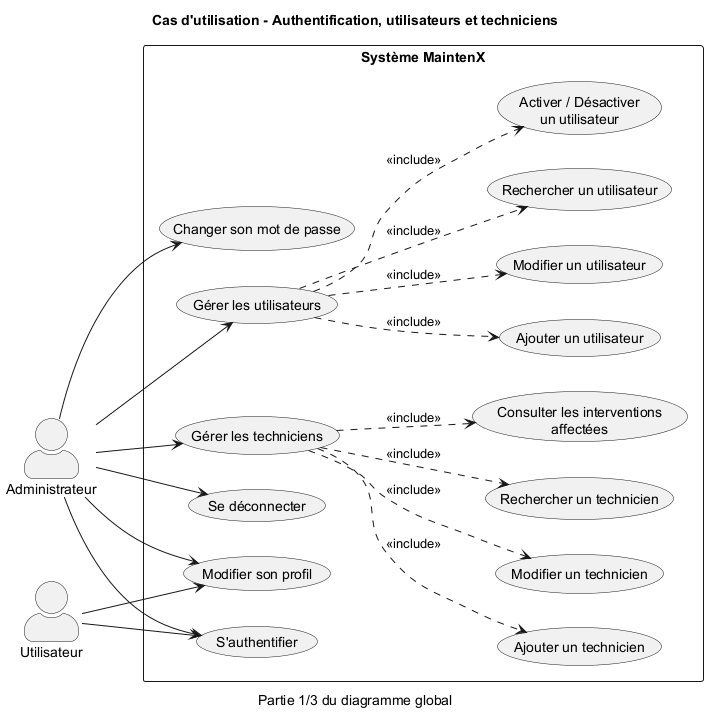
\includegraphics[width=0.925\textwidth]{../../uml/usecase/uc_global_part1.png}
\caption{Cas d'utilisation global --- partie 1/3 (authentification, utilisateurs, techniciens)}
\end{figure}
\begin{figure}[htbp]\centering
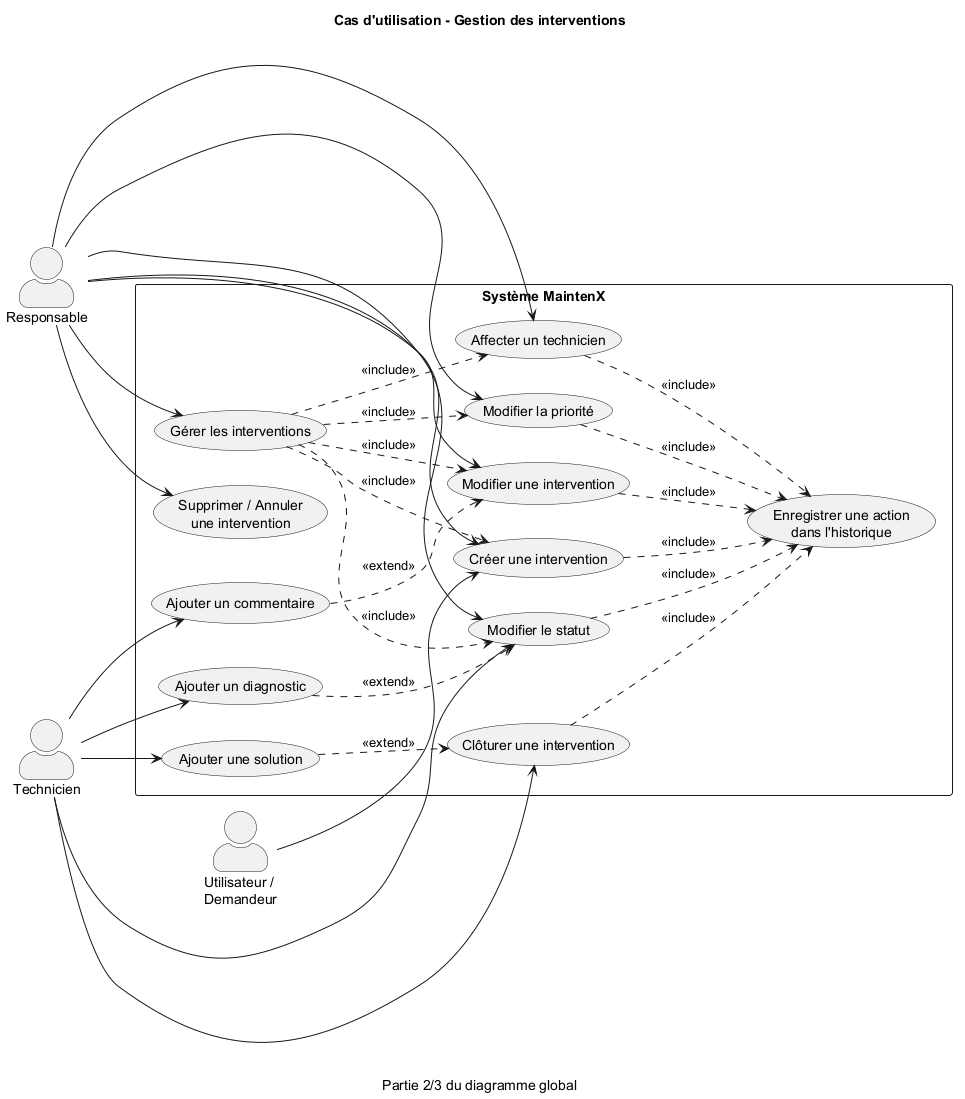
\includegraphics[width=0.925\textwidth]{../../uml/usecase/uc_global_part2.png}
\caption{Cas d'utilisation global --- partie 2/3 (gestion des interventions)}
\end{figure}
\begin{figure}[htbp]\centering
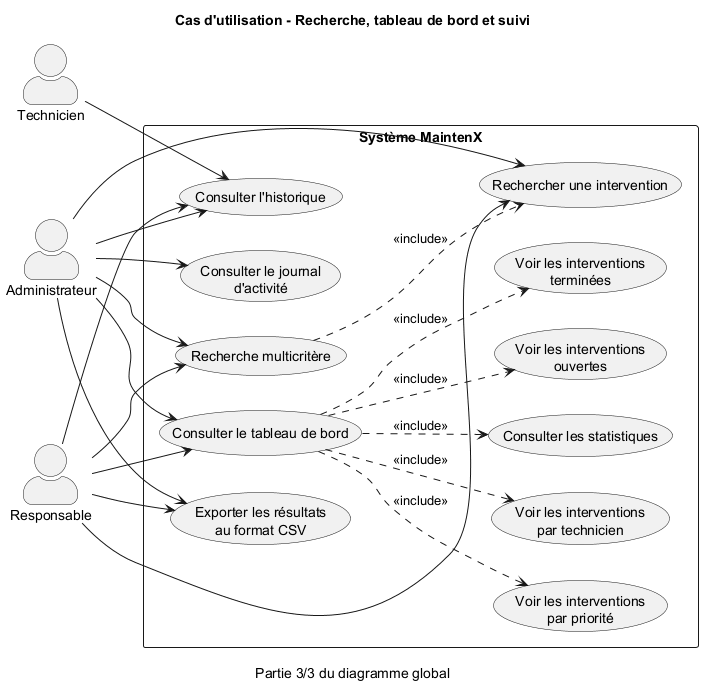
\includegraphics[width=0.925\textwidth]{../../uml/usecase/uc_global_part3.png}
\caption{Cas d'utilisation global --- partie 3/3 (recherche, tableau de bord, suivi)}
\end{figure}

Pour faciliter encore la lecture, des diagrammes par acteur ont également été produits.
\begin{figure}[htbp]\centering
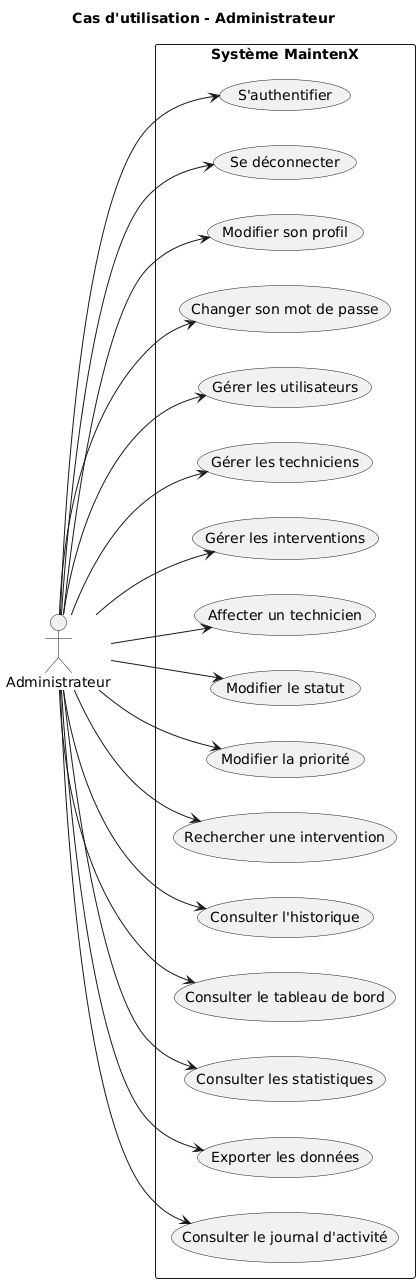
\includegraphics[width=0.436\textwidth]{../../uml/usecase/usecase.admin.png}
\caption{Cas d'utilisation - Administrateur}
\end{figure}
\begin{figure}[htbp]\centering
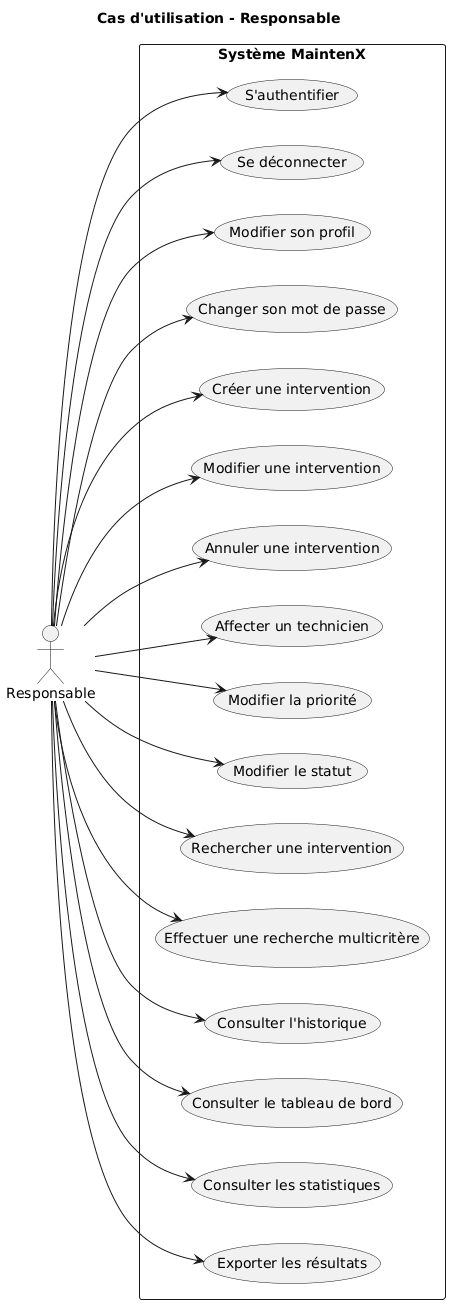
\includegraphics[width=0.460\textwidth]{../../uml/usecase/usecaserespo.png}
\caption{Cas d'utilisation - Responsable}
\end{figure}
\begin{figure}[htbp]\centering
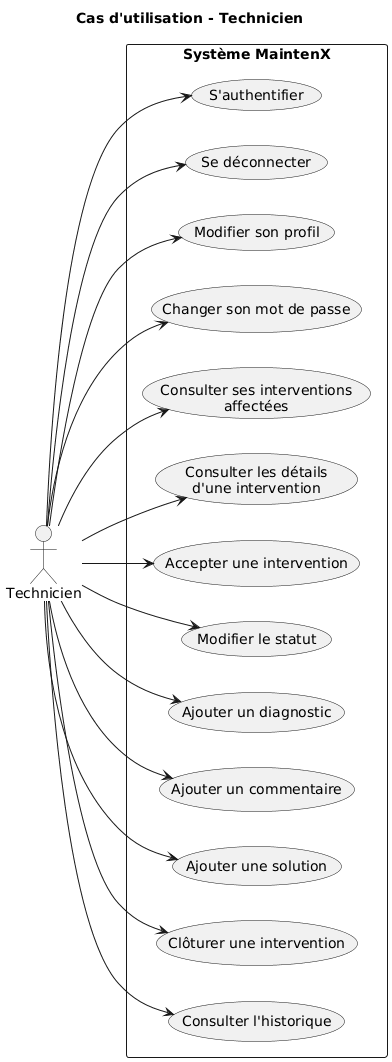
\includegraphics[width=0.492\textwidth]{../../uml/usecase/usecasetechicien.png}
\caption{Cas d'utilisation - Technicien}
\end{figure}
\begin{figure}[htbp]\centering
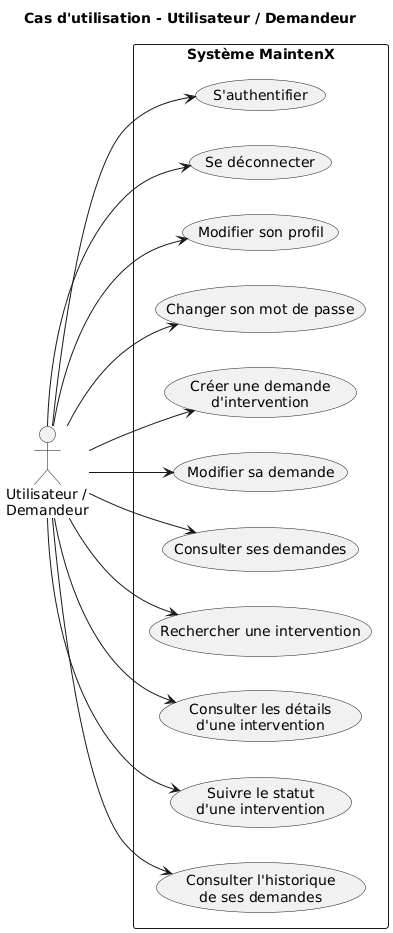
\includegraphics[width=0.561\textwidth]{../../uml/usecase/uscaseusers.png}
\caption{Cas d'utilisation - Gestion des utilisateurs (détail)}
\end{figure}

On note que le cas \textbf{S'authentifier} est préalable à toutes les autres interactions : l'authentification est donc la porte d'entrée du système. Les cas de gestion (utilisateurs, techniciens, interventions) incluent systématiquement l'\textbf{enregistrement dans l'historique}, ce qui matérialise l'exigence de traçabilité.
\phantomsection
\section*{2.3. Diagramme de classes}
\addcontentsline{toc}{section}{2.3. Diagramme de classes}

Le \textbf{diagramme de classes} représente la structure statique du système : les entités métier, leurs attributs, leurs associations et les interfaces qui définissent les contrats des couches.
\begin{figure}[htbp]\centering
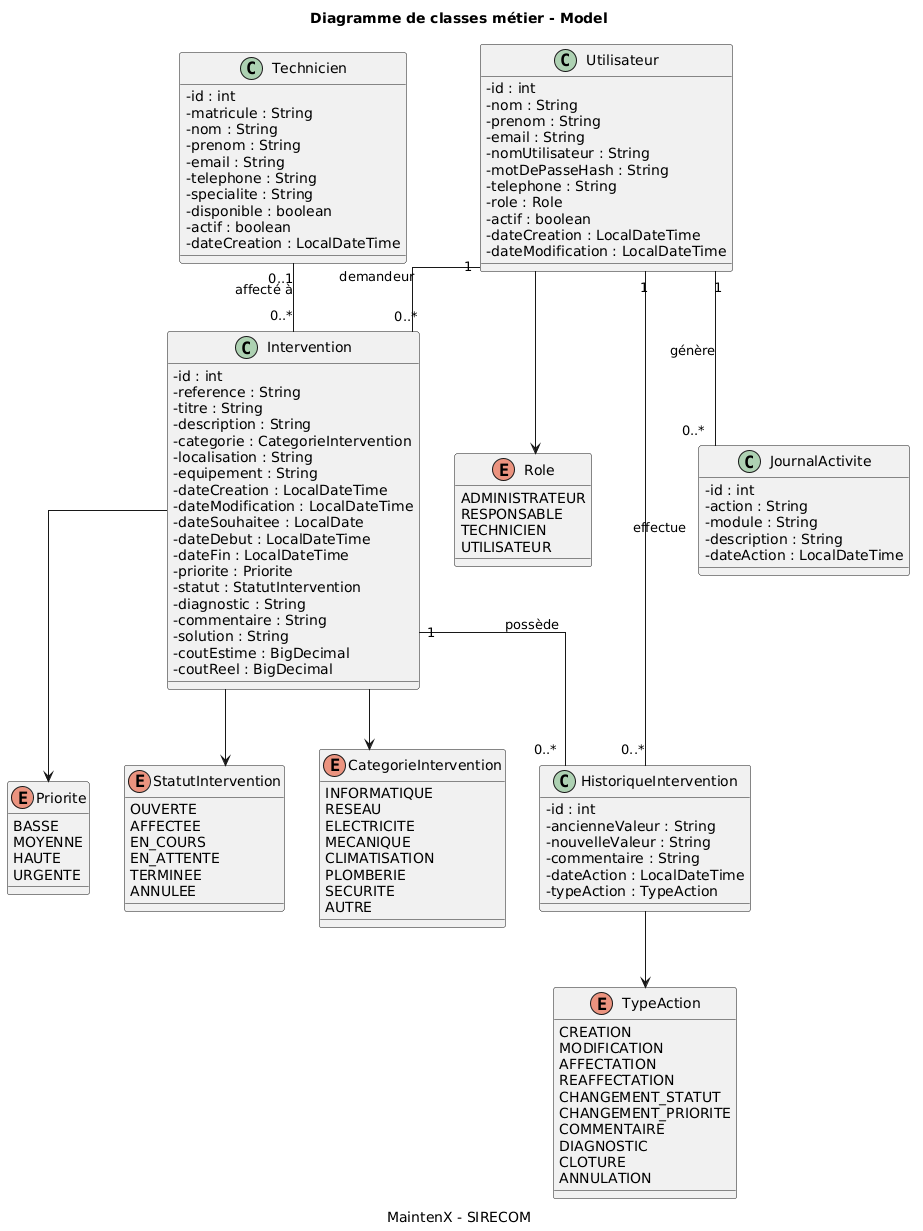
\includegraphics[width=0.925\textwidth]{../../uml/classe/Diagramme de classes métier.png}
\caption{Diagramme des classes métier}
\end{figure}

Les classes métier principales sont :
\begin{itemize}
  \item \textbf{Utilisateur} : compte de connexion (nom, prénom, email, nom d'utilisateur, mot de passe haché, rôle, téléphone, actif) ;
  \item \textbf{Technicien} : agent d'intervention (matricule, nom, prénom, email, spécialité, disponibilité, interventions en cours) ;
  \item \textbf{Intervention} : entité centrale (référence, titre, description, catégorie, localisation, équipement, dates, priorité, statut, coûts, diagnostic, solution) ;
  \item \textbf{HistoriqueIntervention} : trace des actions réalisées sur une intervention (action, ancienne et nouvelle valeur, utilisateur, date) ;
  \item \textbf{JournalActivite} : journal global des connexions et des actions du système.
\end{itemize}

Les \textbf{enums} \textbf{Role}, \textbf{Priorite}, \textbf{StatutIntervention} et \textbf{Specialite} permettent de limiter les valeurs possibles et d'éviter les incohérences.
\begin{table}[htbp]\centering\small
\begin{tabularx}{\textwidth}{|p{3.8cm}|X|}
\hline\rowcolor{hdr}\textbf{Classe / Interface} & \textbf{Rôle dans l'architecture}\\ \hline
Utilisateur & Compte de connexion et demandeur potentiel\\ \hline
Technicien & Agent réalisant les interventions\\ \hline
Intervention & Entité centrale du domaine (demande de maintenance)\\ \hline
HistoriqueIntervention & Trace chronologique des actions sur une intervention\\ \hline
JournalActivite & Journal global des connexions et actions\\ \hline
GenericDAO<T, ID> & Contrat générique de persistance (CRUD)\\ \hline
UtilisateurService & Règles métier des comptes (unicité, désactivation)\\ \hline
InterventionService & Cycle de vie, affectation, statuts, coûts\\ \hline
AuthenticationService & Vérification des identifiants (BCrypt) et gestion de session\\ \hline
DashboardService & Calcul des statistiques du tableau de bord\\ \hline
\end{tabularx}
\caption{Principales classes et leurs responsabilités}
\end{table}
\begin{figure}[htbp]\centering
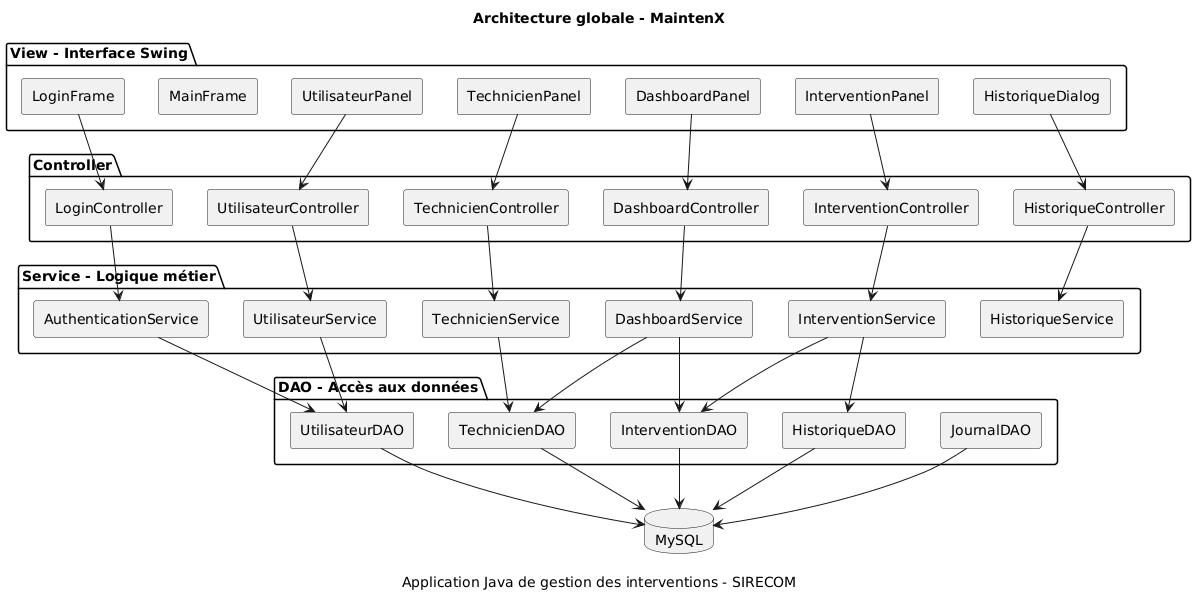
\includegraphics[width=0.925\textwidth]{../../uml/classe/archiglobal.png}
\caption{Architecture globale des classes}
\end{figure}
\begin{figure}[htbp]\centering
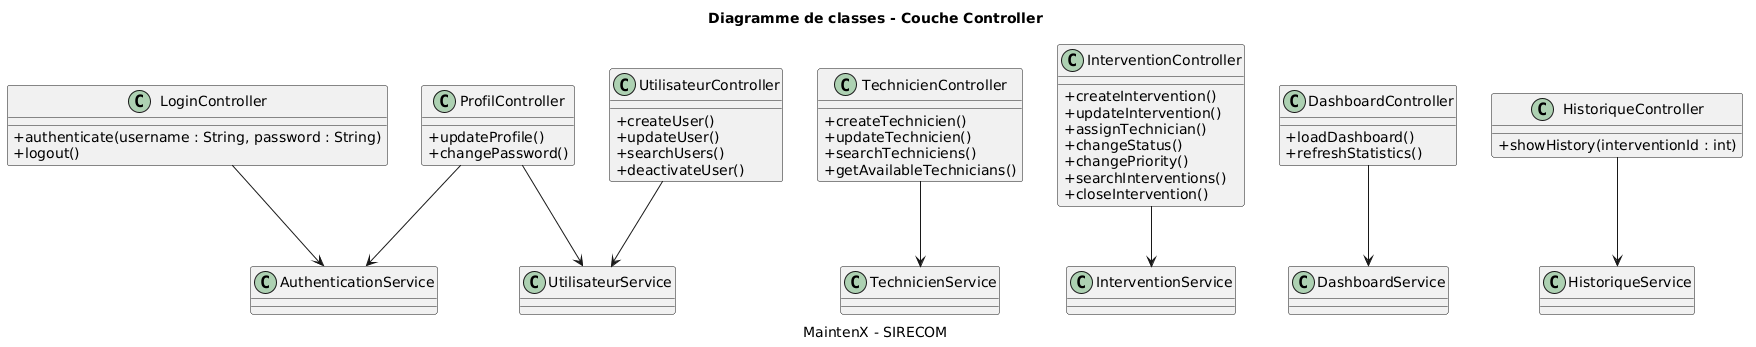
\includegraphics[width=0.925\textwidth]{../../uml/classe/classes Controller.png}
\caption{Diagramme des classes Controller}
\end{figure}
\begin{figure}[htbp]\centering
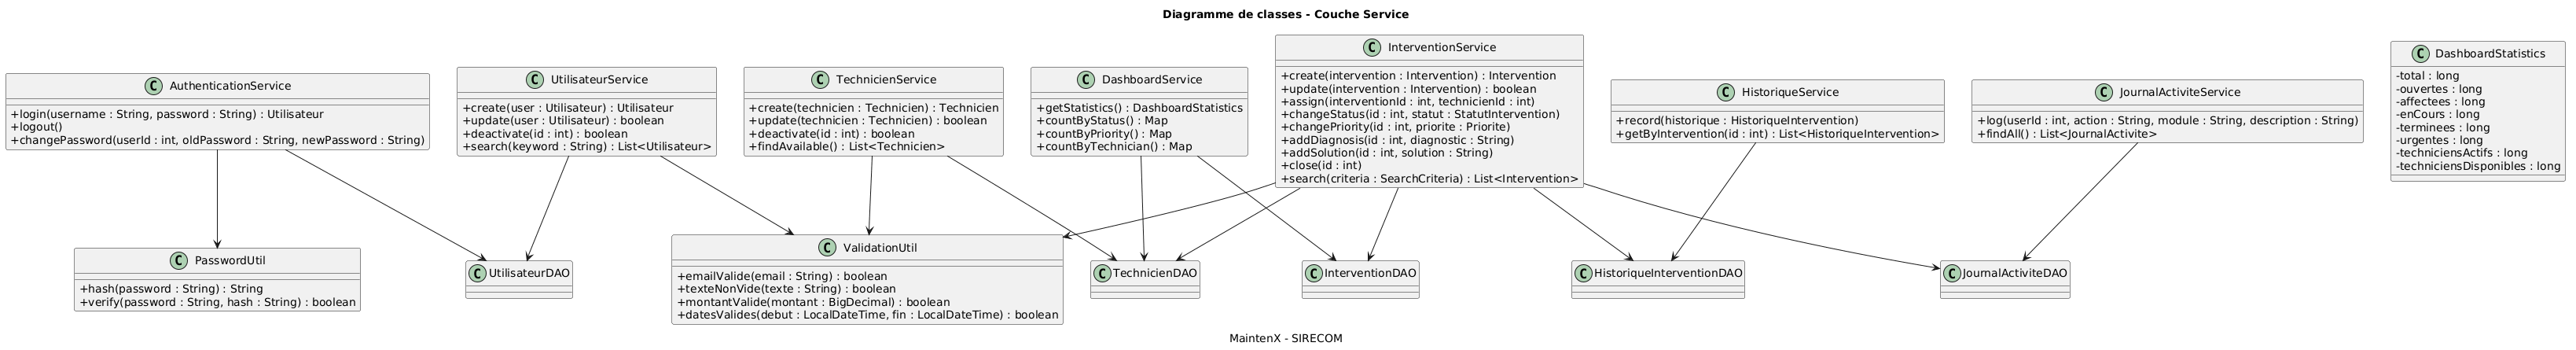
\includegraphics[width=0.925\textwidth]{../../uml/classe/classes Service.png}
\caption{Diagramme des classes Service}
\end{figure}
\begin{figure}[htbp]\centering
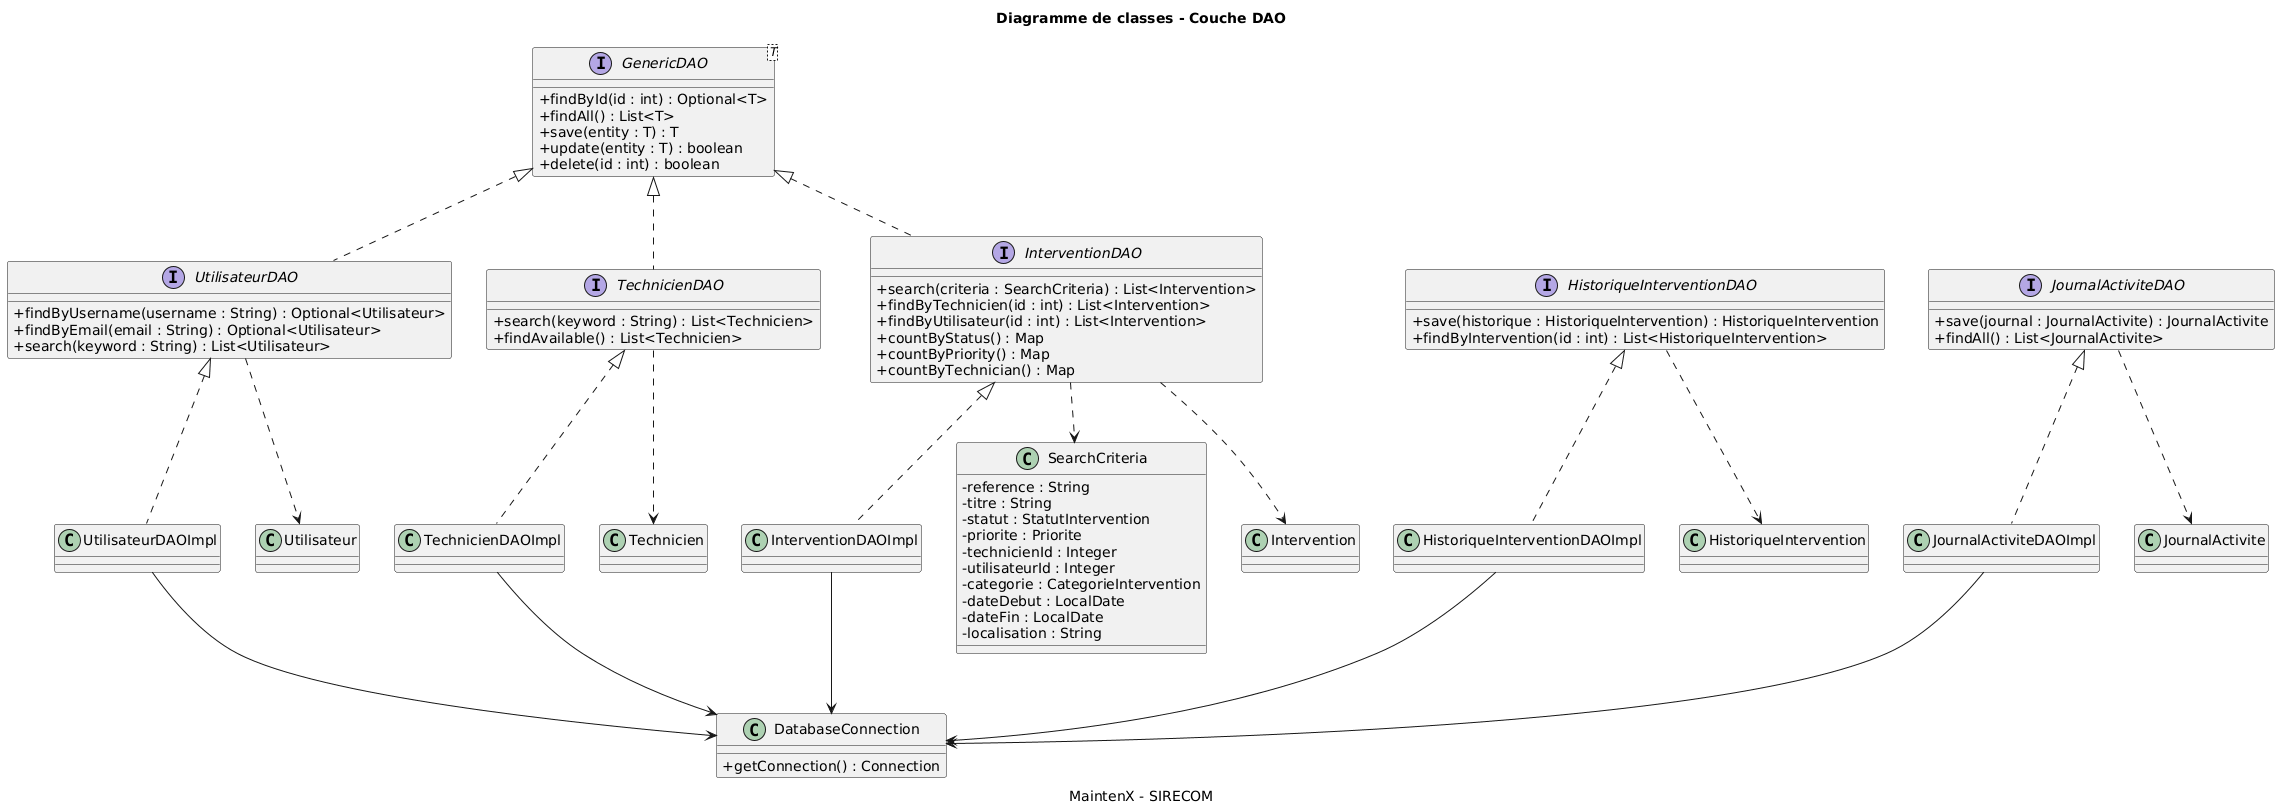
\includegraphics[width=0.925\textwidth]{../../uml/classe/Diagramme des classes DAO.png}
\caption{Diagramme des classes DAO}
\end{figure}

L'interface générique \textbf{GenericDAO<T, ID>} définit les opérations de base (create, update, delete, findById, findAll). Chaque DAO spécialisé étend ce contrat et ajoute ses méthodes propres (recherche, génération de référence, unicité…).
\phantomsection
\section*{2.4. Diagrammes de séquence}
\addcontentsline{toc}{section}{2.4. Diagrammes de séquence}

Les \textbf{diagrammes de séquence} décrivent l'enchaînement temporel des messages échangés entre les objets pour réaliser un cas d'utilisation. Les principaux scénarios sont présentés ci-après.
\phantomsection
\subsection*{2.4.1. Authentification}
\addcontentsline{toc}{subsection}{2.4.1. Authentification}

L'utilisateur saisit ses identifiants dans la \textbf{LoginFrame}. Le \textbf{LoginController} délègue la vérification à l'\textbf{AuthenticationService}, qui journalise la connexion puis ouvre la session dans la \textbf{MainFrame}. Le hachage BCrypt permet de comparer le mot de passe saisi avec le condensat stocké, sans jamais manipuler le mot de passe en clair.
\phantomsection
\subsection*{2.4.2. Création d'une intervention}
\addcontentsline{toc}{subsection}{2.4.2. Création d'une intervention}

Le responsable remplit le formulaire ; le \textbf{InterventionPanel} transmet l'objet au \textbf{InterventionController}, qui appelle la couche service. Le service valide les données, génère la référence unique, enregistre l'événement dans l'historique et renvoie l'intervention créée.
\phantomsection
\subsection*{2.4.3. Affectation d'un technicien}
\addcontentsline{toc}{subsection}{2.4.3. Affectation d'un technicien}

L'affectation vérifie d'abord l'éligibilité du technicien (actif et disponible) via le \textbf{TechnicienService}, met à jour le statut de l'intervention vers \textbf{AFFECTEE}, puis trace l'action dans l'historique.
\phantomsection
\subsection*{2.4.4. Changement de statut et clôture}
\addcontentsline{toc}{subsection}{2.4.4. Changement de statut et clôture}
\begin{figure}[htbp]\centering
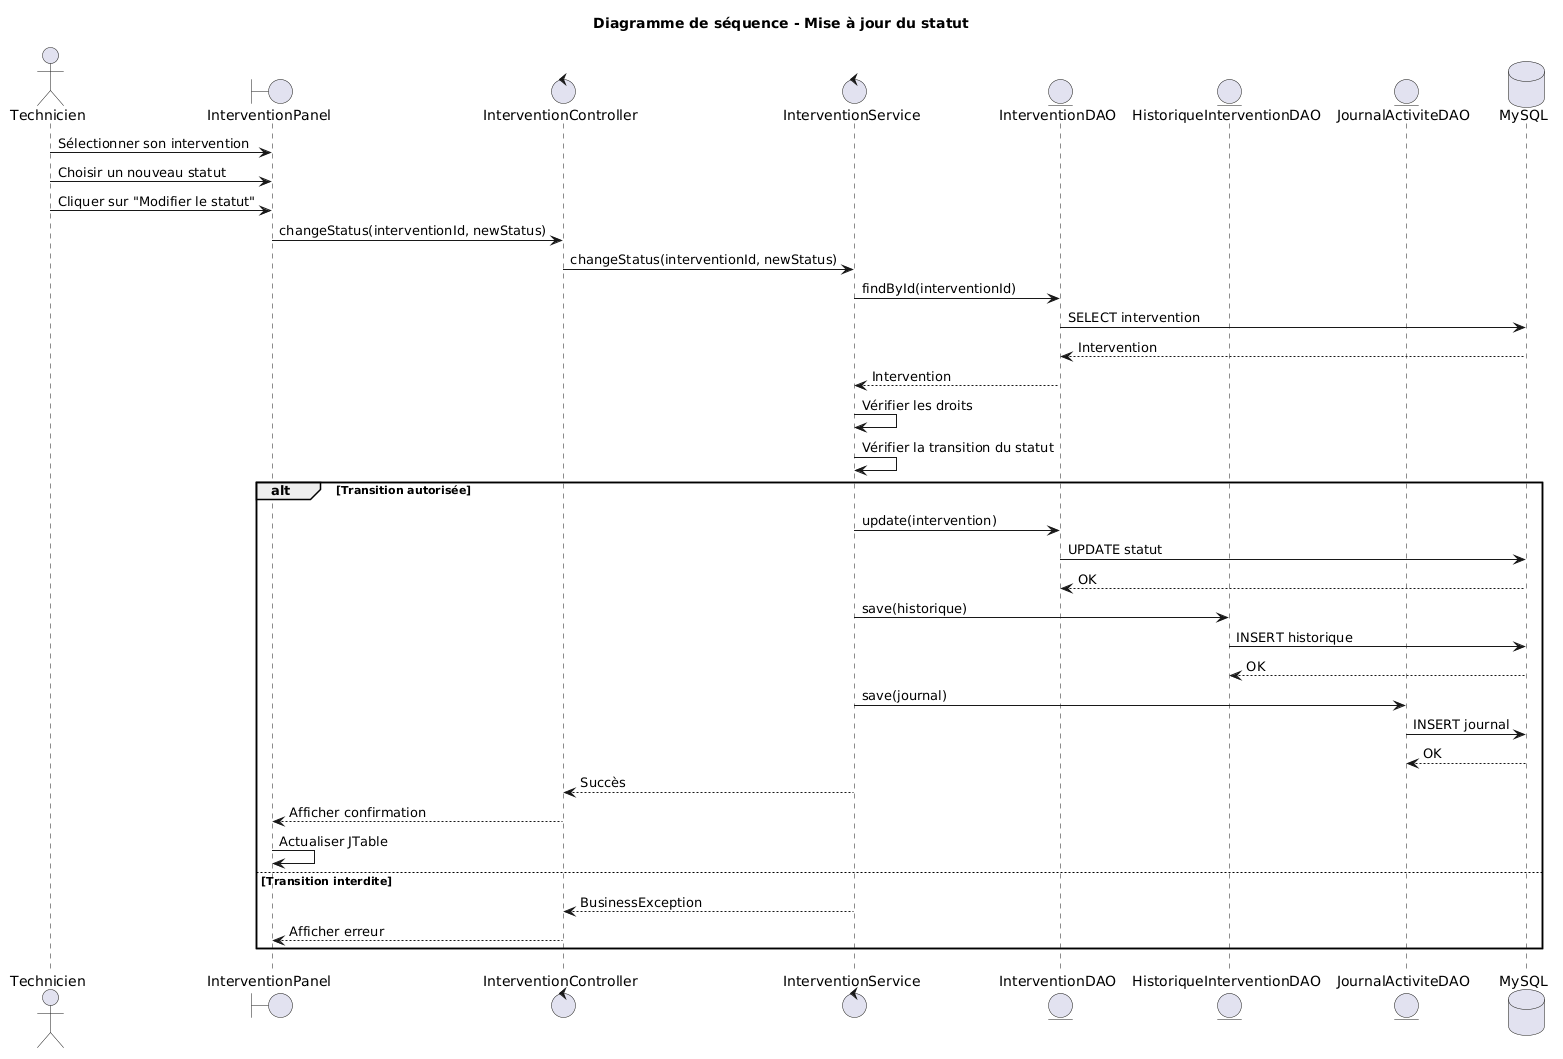
\includegraphics[width=0.894\textwidth]{../../uml/seq/sequences mjrstatut.png}
\caption{Diagramme de séquence - Changement de statut}
\end{figure}

Le changement de statut est soumis aux règles métier : la clôture (\textbf{TERMINEE}) impose une solution appliquée, l'annulation est possible tant que l'intervention n'est pas terminée. Chaque transition alimente l'historique.
\phantomsection
\subsection*{2.4.5. Autres scénarios}
\addcontentsline{toc}{subsection}{2.4.5. Autres scénarios}
\begin{figure}[htbp]\centering
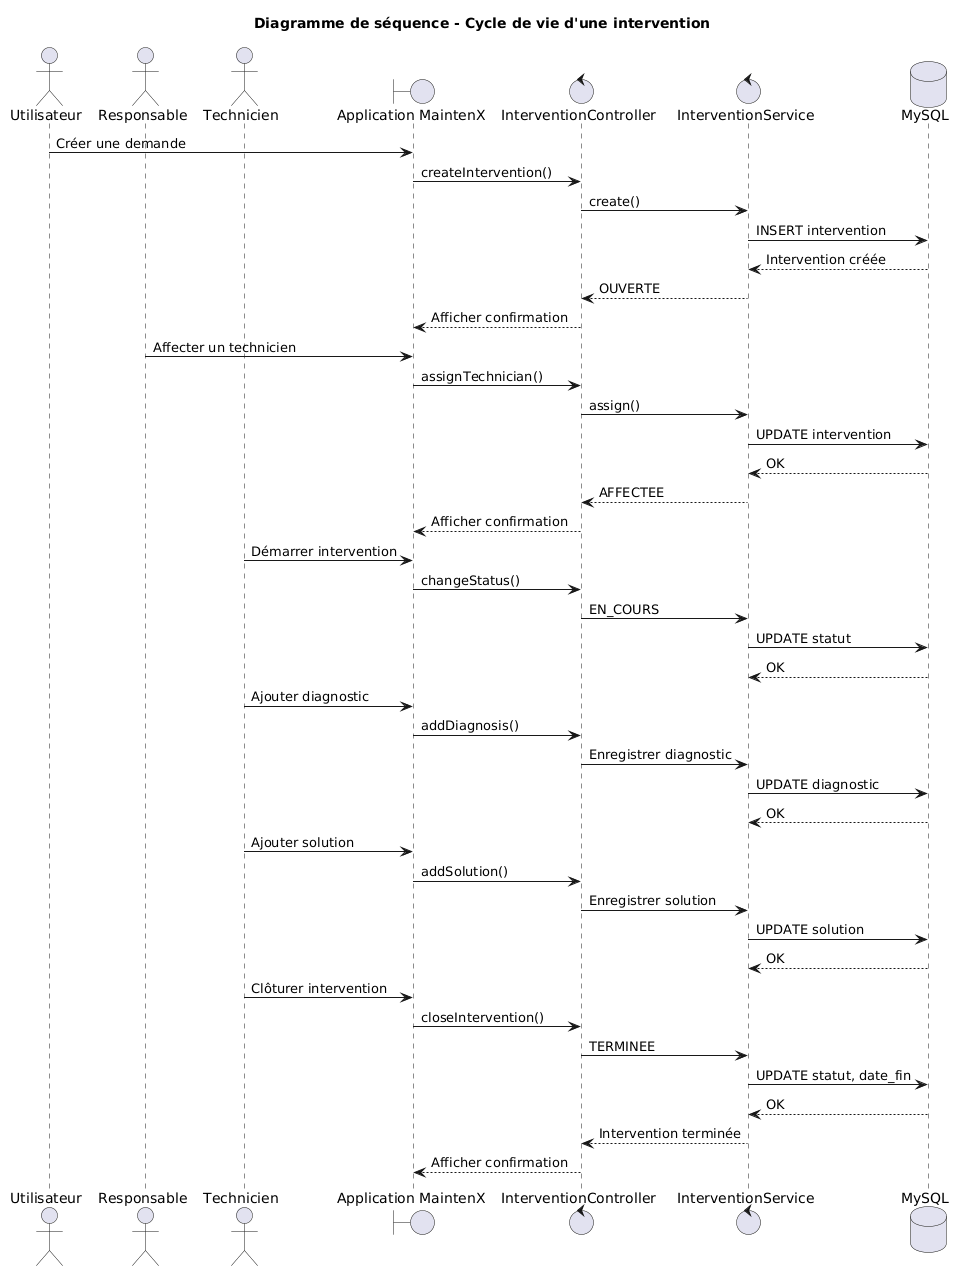
\includegraphics[width=0.894\textwidth]{../../uml/seq/Séquence globale du cycle de vie d'une intervention.png}
\caption{Diagramme de séquence - Cycle de vie global d'une intervention}
\end{figure}

L'analyse des diagrammes de séquence fait ressortir plusieurs propriétés importantes du système :
\begin{itemize}
  \item \textbf{Indépendance des couches} : les objets de la présentation ne dialoguent jamais directement avec la couche de données ; tous les échanges transitent par le contrôleur puis par le service, ce qui rend chaque scénario testable isolément ;
  \item \textbf{Traçabilité systématique} : quelle que soit l'action métier, un message est envoyé au service d'historique (ou au journal) ; il n'existe pas de scénario qui modifie l'état sans laisser de trace ;
  \item \textbf{Validation au plus près du métier} : les conditions (technicien actif et disponible, solution obligatoire, droits de l'acteur) sont vérifiées dans la couche service, pas dans l'interface, ce qui interdit tout contournement.
\end{itemize}

Cette conception garantit que l'application conserve un \textbf{comportement cohérent} même si de nouveaux points d'entrée (par exemple une future version web) sont ajoutés par la suite.
\phantomsection
\subsection*{2.4.6. Vérification de la cohérence du modèle}
\addcontentsline{toc}{subsection}{2.4.6. Vérification de la cohérence du modèle}

Une étape de \textbf{relecture croisée} a été menée en fin de conception afin de vérifier la cohérence entre les différents diagrammes : chaque cas d'utilisation important possède au moins un diagramme de séquence, chaque classe du diagramme de classes a une correspondance dans le MCD et dans l'implémentation, et chaque règle de gestion du cahier des charges est rattachée à un point de contrôle de la couche service. Cette revue a permis de détecter, en amont de l'implémentation, des incohérences de cardinalité (affectation d'un technicien sans vérification de disponibilité) qui ont été corrigées dans le modèle puis appliquées dans le code.
\phantomsection
\section*{2.5. Diagrammes d'activité et d'états}
\addcontentsline{toc}{section}{2.5. Diagrammes d'activité et d'états}

Le \textbf{diagramme d'activité} du cycle de vie d'une intervention représente le flot d'exécution depuis la création jusqu'à la clôture ou l'annulation.

Le \textbf{diagramme d'états} ci-dessous matérialise les transitions autorisées entre les six statuts possibles.
\begin{table}[htbp]\centering\small
\begin{tabularx}{\textwidth}{|X|X|X|}
\hline\rowcolor{hdr}\textbf{Transition} & \textbf{Condition} & \textbf{Acteur autorisé}\\ \hline
OUVERTE $\rightarrow$ AFFECTEE & Technicien actif et disponible sélectionné & Administrateur, Responsable\\ \hline
AFFECTEE $\rightarrow$ EN\_COURS & Début de l'intervention & Technicien affecté\\ \hline
EN\_COURS $\rightarrow$ EN\_ATTENTE & Blocage (pièce, information) & Technicien affecté\\ \hline
EN\_ATTENTE $\rightarrow$ EN\_COURS & Levée du blocage & Technicien affecté\\ \hline
EN\_COURS $\rightarrow$ TERMINEE & Solution appliquée obligatoire & Technicien affecté\\ \hline
OUVERTE $\rightarrow$ ANNULEE & Demande annulée & Administrateur, Responsable\\ \hline
\end{tabularx}
\caption{Transitions de statut autorisées}
\end{table}
\phantomsection
\section*{2.6. Diagrammes de composants et de déploiement}
\addcontentsline{toc}{section}{2.6. Diagrammes de composants et de déploiement}
\begin{figure}[htbp]\centering
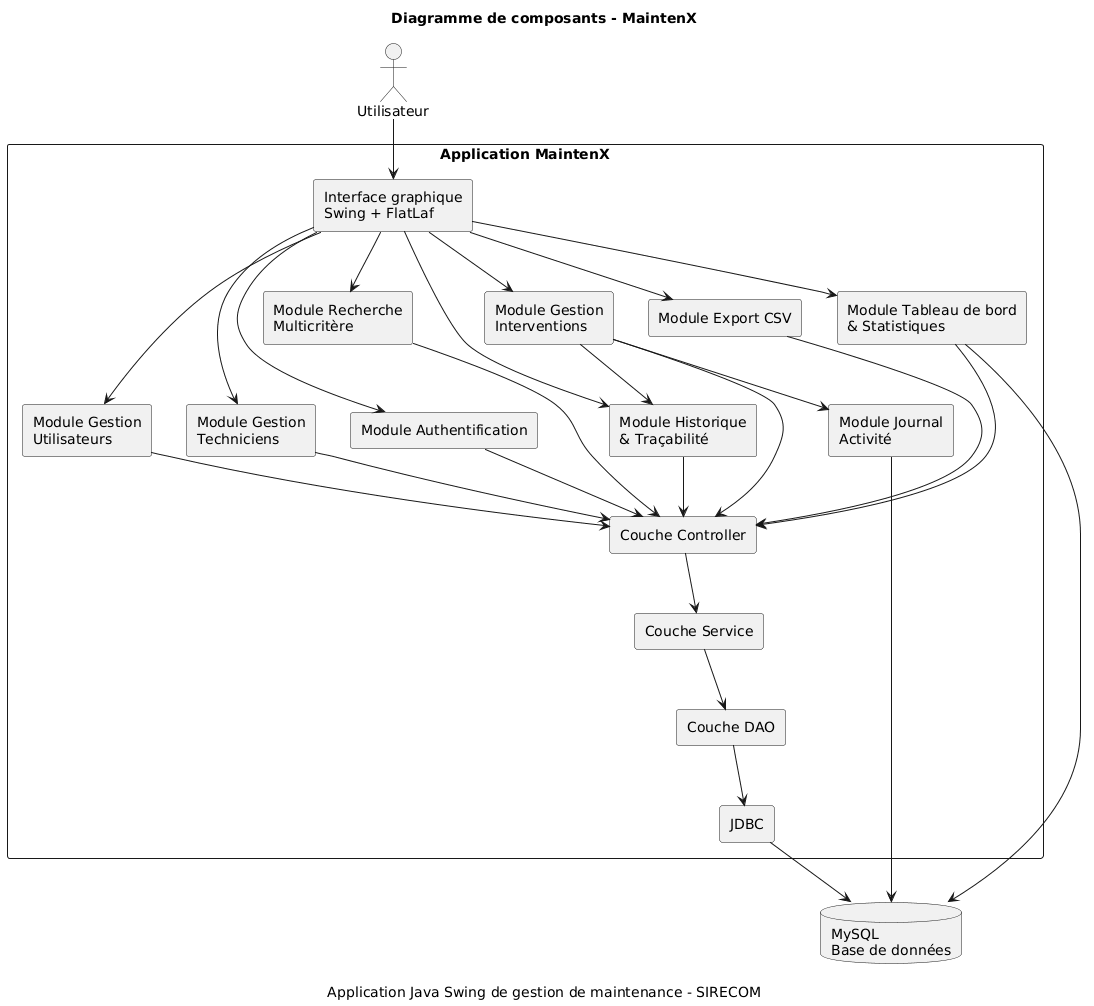
\includegraphics[width=0.894\textwidth]{../../uml/Diagramme de composants.png}
\caption{Diagramme de composants}
\end{figure}

Le diagramme de composants montre la dépendance unidirectionnelle entre les couches : les vues Swing dépendent des contrôleurs, lesquels s'appuient sur les services métier, eux-mêmes adossés aux DAO qui communiquent avec MySQL via JDBC.
\begin{figure}[htbp]\centering
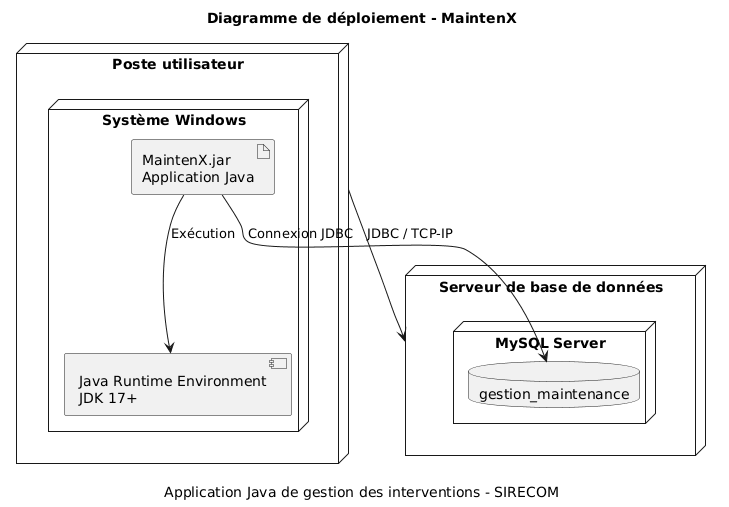
\includegraphics[width=0.894\textwidth]{../../uml/Diagramme de déploiement.png}
\caption{Diagramme de déploiement}
\end{figure}

Le déploiement est simple : le JAR exécutable \textbf{maintenx.jar} est déployé sur le poste utilisateur et se connecte, par JDBC, à la base \textbf{gestion\_maintenance} hébergée par un serveur MySQL. En mode démonstration, aucune connexion n'est requise, les données étant chargées en mémoire.
\phantomsection
\section*{2.7. Modèle Conceptuel de Données (MCD)}
\addcontentsline{toc}{section}{2.7. Modèle Conceptuel de Données (MCD)}

Le \textbf{Modèle Conceptuel de Données} formalise les entités et les associations de la base. Le modèle retenu comprend six entités : \textbf{utilisateur}, \textbf{technicien}, \textbf{intervention}, \textbf{historique\_intervention}, \textbf{journal\_activite} et \textbf{parametre\_application}.
\begin{figure}[htbp]\centering
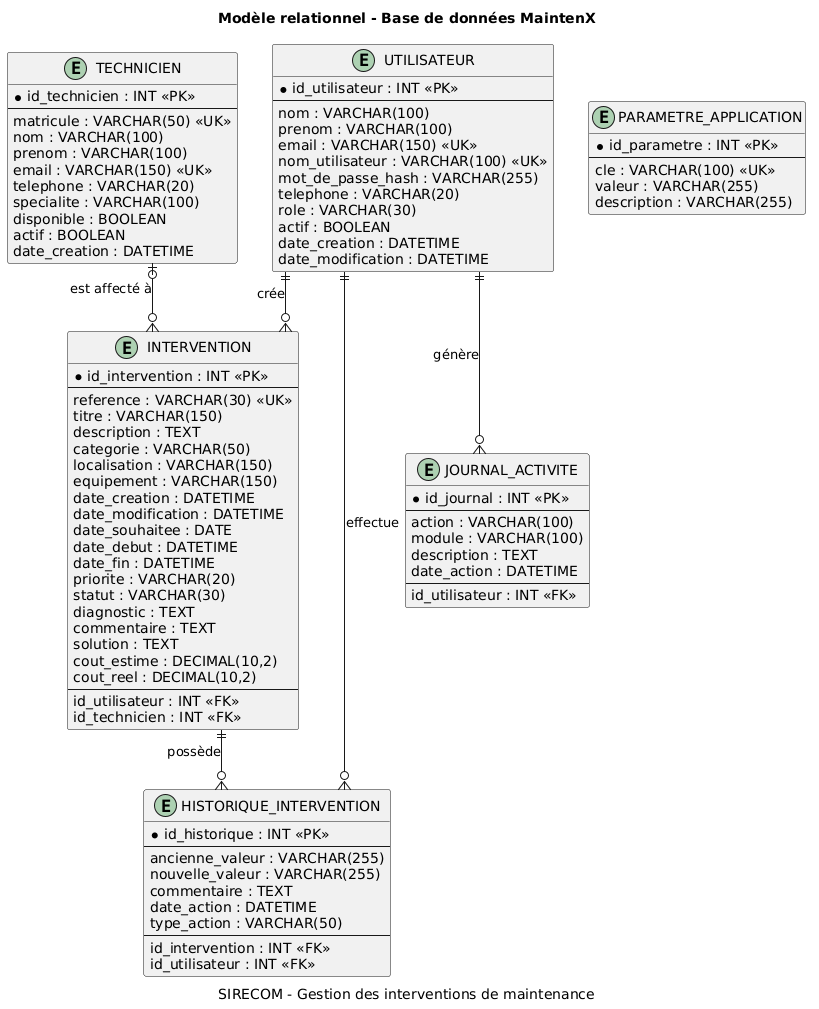
\includegraphics[width=0.925\textwidth]{../../uml/MCD.PNG}
\caption{Modèle Conceptuel de Données (MCD)}
\end{figure}

Les principales associations sont : un utilisateur peut émettre plusieurs interventions (\textbf{demandeur}), un technicien peut être affecté à plusieurs interventions, et une intervention possède plusieurs lignes d'historique. La cardinalité (0,1)-(0,n) sur l'affectation traduit le fait qu'une intervention peut ne pas encore avoir de technicien.
\phantomsection
\subsection*{2.7.1. Schéma relationnel (notation)}
\addcontentsline{toc}{subsection}{2.7.1. Schéma relationnel (notation)}

Le passage du MCD au \textbf{schéma relationnel} applique les règles classiques de transformation : chaque entité devient une relation (table), et chaque association est matérialisée par une \textbf{clé étrangère}. Dans la notation retenue, la clé primaire est le premier attribut (elle serait soulignée dans la notation classique) et les clés étrangères sont précédées du symbole \textbf{\#} :
\begin{lstlisting}
UTILISATEUR (id, nom, prénom, email, nom_utilisateur, mot_de_passe_hash,
            rôle, téléphone, actif, date_creation, date_modification)
TECHNICIEN (id, matricule, nom, prénom, email, téléphone, spécialité,
            disponible, actif, interventions_en_cours, date_creation)
INTERVENTION (id, référence, titre, description, catégorie, localisation,
              équipement, date_creation, date_modification, date_souhaitée,
              date_début, date_fin, priorité, statut,
              #demandeur_id, #technicien_id, commentaire, diagnostic,
              solution_appliquée, coût_estimé, coût_réel)
HISTORIQUE_INTERVENTION (id, #intervention_id, action, ancienne_valeur,
                         nouvelle_valeur, utilisateur, date_action)
JOURNAL_ACTIVITE (id, utilisateur, action, détails, date_action)
PARAMETRE_APPLICATION (clé, valeur, date_modification)
\end{lstlisting}

Chaque relation possède une \textbf{clé primaire} (`id`, ou `clé` pour `parametre\_application`). Les \textbf{clés étrangères} traduisent les associations du MCD : `demandeur\_id` référence `utilisateur(id)` (un demandeur peut être à l'origine de plusieurs interventions), `technicien\_id` référence `technicien(id)` (affectation d'un technicien), et `intervention\_id` référence `intervention(id)` (traçabilité des actions). Aucune association plusieurs-à-plusieurs ne nécessite de table de liaison : le modèle reste simple et directement exploitable en SQL.
\begin{table}[htbp]\centering\small
\begin{tabularx}{\textwidth}{|X|X|X|}
\hline\rowcolor{hdr}\textbf{Relation} & \textbf{Clé primaire} & \textbf{Clés étrangères (références)}\\ \hline
utilisateur & id & ---\\ \hline
technicien & id & ---\\ \hline
intervention & id & demandeur\_id $\rightarrow$ utilisateur(id) ; technicien\_id $\rightarrow$ technicien(id)\\ \hline
historique\_intervention & id & intervention\_id $\rightarrow$ intervention(id)\\ \hline
journal\_activite & id & ---\\ \hline
parametre\_application & clé & ---\\ \hline
\end{tabularx}
\caption{Récapitulatif des relations et de leurs contraintes}
\end{table}
\phantomsection
\subsection*{2.7.2. Dictionnaire de données (extrait)}
\addcontentsline{toc}{subsection}{2.7.2. Dictionnaire de données (extrait)}

Le dictionnaire de données complet est fourni dans la documentation technique. Les extraits ci-dessous décrivent les tables principales.
\begin{table}[htbp]\centering\small
\begin{tabularx}{\textwidth}{|X|X|X|X|}
\hline\rowcolor{hdr}\textbf{Champ} & \textbf{Type} & \textbf{Contrainte} & \textbf{Description}\\ \hline
utilisateur.id & BIGINT & PK, auto & Identifiant\\ \hline
utilisateur.email & VARCHAR(160) & UNIQUE & Adresse électronique\\ \hline
utilisateur.nom\_utilisateur & VARCHAR(80) & UNIQUE & Identifiant de connexion\\ \hline
utilisateur.mot\_de\_passe\_hash & VARCHAR(255) & Obligatoire & Condensat BCrypt\\ \hline
utilisateur.role & ENUM & Obligatoire & Rôle (ADMINISTRATEUR, RESPONSABLE, TECHNICIEN)\\ \hline
technicien.matricule & VARCHAR(40) & UNIQUE & Matricule\\ \hline
technicien.specialite & ENUM & Obligatoire & Domaine d'intervention\\ \hline
intervention.reference & VARCHAR(30) & UNIQUE & Référence INT-AAAA-NNNN\\ \hline
intervention.priorite & ENUM & INDEX & BASSE / MOYENNE / HAUTE / URGENTE\\ \hline
intervention.statut & ENUM & INDEX & Cycle de vie\\ \hline
intervention.cout\_estime & DECIMAL(12,2) & >= 0 & Coût estimé\\ \hline
intervention.cout\_reel & DECIMAL(12,2) & >= 0 (CHECK) & Coût réel\\ \hline
historique\_intervention.action & VARCHAR(80) & Obligatoire & Action tracée\\ \hline
journal\_activite.action & VARCHAR(100) & Obligatoire & Action globale\\ \hline
\end{tabularx}
\caption{Dictionnaire de données (extrait)}
\end{table}
\phantomsection
\subsection*{2.7.3. Le schéma relationnel (script SQL)}
\addcontentsline{toc}{subsection}{2.7.3. Le schéma relationnel (script SQL)}

Le schéma relationnel est directement déduit du MCD. Le script de création, fourni dans `database/schema.sql`, est rappelé ci-dessous pour la table centrale de l'application :
\begin{lstlisting}
CREATE TABLE intervention (
  id BIGINT PRIMARY KEY AUTO_INCREMENT,
  reference VARCHAR(30) NOT NULL UNIQUE,
  titre VARCHAR(180) NOT NULL,
  description TEXT NOT NULL,
  categorie VARCHAR(80) NOT NULL,
  localisation VARCHAR(160) NOT NULL,
  equipement VARCHAR(160),
  date_creation DATETIME NOT NULL DEFAULT CURRENT_TIMESTAMP,
  date_souhaitee DATE,
  date_debut DATETIME,
  date_fin DATETIME,
  priorite ENUM('BASSE','MOYENNE','HAUTE','URGENTE')
            NOT NULL DEFAULT 'MOYENNE',
  statut ENUM('OUVERTE','AFFECTEE','EN_COURS','EN_ATTENTE',
              'TERMINEE','ANNULEE') NOT NULL DEFAULT 'OUVERTE',
  demandeur_id BIGINT,
  technicien_id BIGINT,
  diagnostic TEXT,
  solution_appliquee TEXT,
  cout_estime DECIMAL(12,2) NOT NULL DEFAULT 0,
  cout_reel DECIMAL(12,2) NOT NULL DEFAULT 0,
  CONSTRAINT fk_intervention_demandeur
      FOREIGN KEY (demandeur_id) REFERENCES utilisateur(id),
  CONSTRAINT fk_intervention_technicien
      FOREIGN KEY (technicien_id) REFERENCES technicien(id),
  CONSTRAINT chk_cout_reel CHECK (cout_reel >= 0),
  INDEX idx_intervention_statut(statut),
  INDEX idx_intervention_priorite(priorite)
) ENGINE=InnoDB DEFAULT CHARSET=utf8mb4;
\end{lstlisting}

Le jeu de caractères \textbf{utf8mb4} et le moteur \textbf{InnoDB} garantissent le support des accents et l'intégrité référentielle. Des \textbf{vues} (`v\_interventions\_detaillees`, `v\_dashboard\_statut`) sont également définies pour simplifier l'exploitation des données (jointures demandeur/technicien, agrégats par statut).

Le script SQL complet (création des tables, clés étrangères, index, vues) est fourni dans le dossier `database/` du projet et reproduit en annexe.
\phantomsection
\chapter*{Chapitre 3 : Réalisation et implémentation}
\addcontentsline{toc}{chapter}{Chapitre 3 : Réalisation et implémentation}
\phantomsection
\section*{3.1. Environnement de développement}
\addcontentsline{toc}{section}{3.1. Environnement de développement}

Le choix des technologies a été guidé par les contraintes du cahier des charges (application de bureau, coût nul de licence, écosystème Java maîtrisé) et par l'objectif de maintenabilité.
\begin{table}[htbp]\centering\small
\begin{tabularx}{\textwidth}{|X|X|X|}
\hline\rowcolor{hdr}\textbf{Catégorie} & \textbf{Technologie / Outil} & \textbf{Rôle}\\ \hline
Langage & Java 25 (OpenJDK Temurin) & Langage principal de l'application\\ \hline
Bibliothèque graphique & Java Swing + FlatLaf & Interface utilisateur et thème moderne (clair/sombre)\\ \hline
Persistance & JDBC (java.sql) & Accès aux données et aux requêtes préparées\\ \hline
SGBD & MySQL 8 (InnoDB, utf8mb4) & Stockage relationnel\\ \hline
Sécurité & jBCrypt & Hachage et vérification des mots de passe\\ \hline
Build & Maven 3.9 + plugin Shade & Compilation, tests, packaging JAR exécutable\\ \hline
Tests & JUnit 5 (Jupiter) & Tests unitaires automatisés\\ \hline
Modélisation & PlantUML & Diagrammes UML (cas d'utilisation, classes, séquences…)\\ \hline
IDE & VS Code / IntelliJ IDEA & Édition et débogage\\ \hline
Documentation & Markdown & Documentation technique et utilisateur\\ \hline
\end{tabularx}
\caption{Environnement de développement}
\end{table}

L'environnement d'exécution cible est un poste Windows équipé d'un JRE 25. La base MySQL peut être fournie par une installation locale (XAMPP ou MySQL Server) ou distante.
\phantomsection
\subsection*{3.1.1. Justification des choix technologiques}
\addcontentsline{toc}{subsection}{3.1.1. Justification des choix technologiques}

Les choix retenus résultent d'un arbitrage entre le cahier des charges, les contraintes de l'entreprise et les bonnes pratiques :
\begin{itemize}
  \item \textbf{Java + Swing} : langage objet robuste et portable ; Swing, bien que moins \guillemotleft{} moderne \guillemotright{} que JavaFX, est stable, sans dépendances lourdes et largement documenté ; il permet de livrer une application autonome très rapidement ;
  \item \textbf{FlatLaf} : thème Look and Feel moderne et personnalisable qui améliore nettement le rendu visuel de Swing (angles arrondis, thème clair/sombre) sans surcharge de développement ;
  \item \textbf{JDBC plutôt qu'un ORM} : le nombre de tables est limité ; l'usage direct de `PreparedStatement` donne un contrôle total sur les requêtes, garantit la protection contre l'injection SQL et évite d'introduire une dépendance externe ;
  \item \textbf{MySQL 8} : SGBD open source, répandu et déjà utilisé par l'entreprise pour ses applications ;
  \item \textbf{Maven} : standard de facto pour la construction Java (dépendances, tests, packaging) ; le plugin Shade produit un JAR autonome, simplifiant le déploiement ;
  \item \textbf{JUnit 5} : cadre de test de référence, intégré nativement à la phase de construction Maven.
\end{itemize}

Le compromis obtenu est une application \textbf{légère, installable sans serveur d'application} et \textbf{facile à faire évoluer}.
\phantomsection
\section*{3.2. Architecture de l'application}
\addcontentsline{toc}{section}{3.2. Architecture de l'application}

MaintenX adopte une \textbf{architecture multicouche} qui sépare strictement les responsabilités : les vues n'appellent jamais directement les DAO, et toutes les règles métier sont centralisées dans les services.
\begin{figure}[htbp]\centering
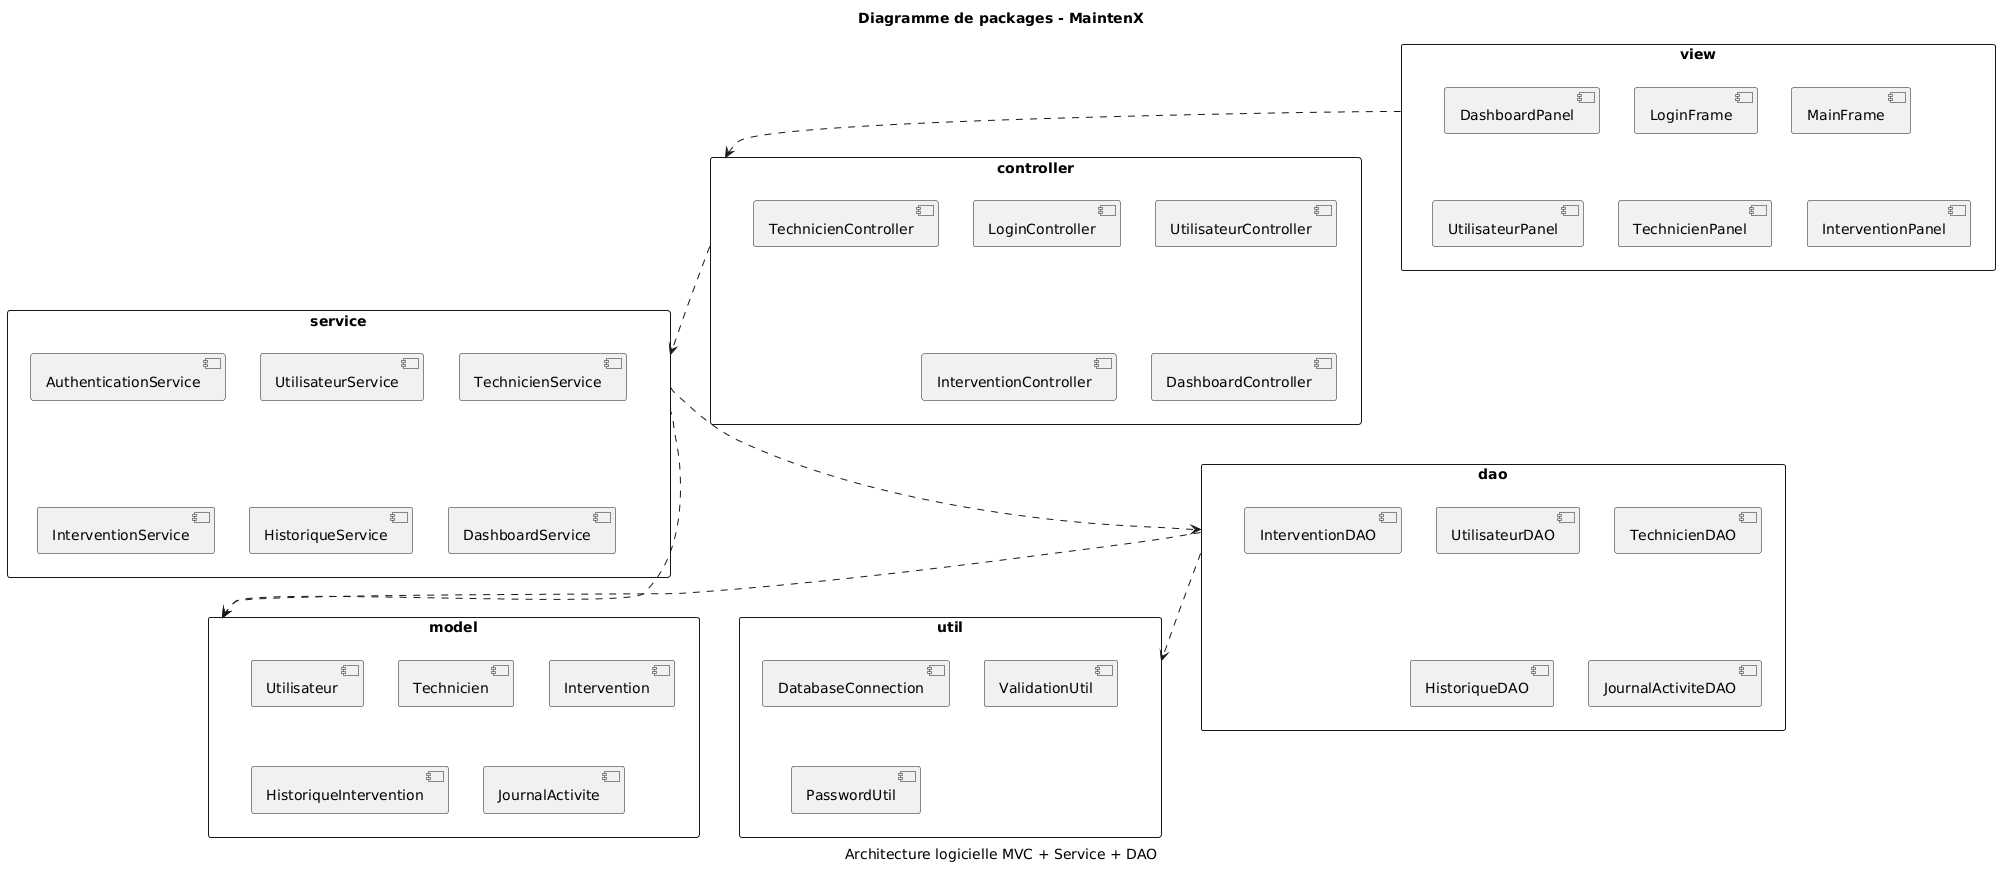
\includegraphics[width=0.894\textwidth]{../../uml/package.png}
\caption{Organisation des packages}
\end{figure}

Le flux de contrôle est le suivant : \textbf{Vue (Swing) $\rightarrow$ Contrôleur $\rightarrow$ Service $\rightarrow$ DAO $\rightarrow$ MySQL}. Ce découpage apporte plusieurs bénéfices : testabilité (les services se testent sans interface graphique), maintenabilité (chaque couche évolue indépendamment), et sécurité (les validations ne dépendent pas de l'interface).
\phantomsection
\subsection*{3.2.1. Structure du projet}
\addcontentsline{toc}{subsection}{3.2.1. Structure du projet}
\begin{lstlisting}
gestion-interventions-maintenance/
+-- pom.xml                          # Configuration Maven
+-- database/                        # Scripts SQL (schema, données, vues)
+-- docs/                            # Documentation (technique, utilisateur, tests, UML)
+-- uml/                             # Diagrammes UML exportés
+-- src/
    +-- main/java/com/maintenx/
    |   +-- Main.java                # Point d'entrée
    |   +-- model/ + model/enums/    # Entités métier et énumérations
    |   +-- view/                    # Frames, panneaux, dialogues, composants
    |   +-- controller/              # Contrôleurs (Login, Intervention, Utilisateur…)
    |   +-- service/ + service/impl/ # Interfaces et implémentations métier
    |   +-- dao/ + dao/impl/         # Contrats de persistance et implémentations JDBC
    |   +-- util/                    # Connexion, config, hachage, erreurs
    |   +-- validation/              # Validations réutilisables
    |   +-- exception/               # Exceptions métier
    +-- main/resources/              # Fichier de configuration (config.properties)
    +-- test/java/                   # Tests unitaires JUnit 5
\end{lstlisting}
\phantomsection
\subsection*{3.2.2. Point d'entrée de l'application}
\addcontentsline{toc}{subsection}{3.2.2. Point d'entrée de l'application}

La classe `Main` initialise l'application : application du thème FlatLaf, chargement des préférences utilisateur, création du magasin de données et des services, puis affichage de l'écran de connexion.
\begin{lstlisting}
public class Main {
    public static void main(String[] args) {
        FlatLightLaf.setup();          // thème par défaut
        AppPreferences.load();        // préférences (thème, fenêtre)
        var store = DemoDataFactory.createStore(); // données démo
        var journal = new JournalActiviteServiceImpl(store);
        var services = Services.factory(store, journal);
        new LoginFrame(services).setVisible(true);
    }
}
\end{lstlisting}

En mode démonstration, `DemoDataFactory` peuple un `InMemoryStore` avec des utilisateurs, des techniciens et des interventions cohérents. Ce mode garantit une présentation fluide même en l'absence de serveur MySQL ; le branchement sur la base réelle est assuré par les DAO JDBC.

Les \textbf{préférences} (thème clair/sombre, dimensions de la fenêtre) sont enregistrées via `java.util.prefs`, ce qui permet de conserver les choix de l'utilisateur entre deux lancements.
\phantomsection
\section*{3.3. Couche modèle}
\addcontentsline{toc}{section}{3.3. Couche modèle}

La couche modèle regroupe les classes métier et les énumérations du domaine. Les classes utilisent des \textbf{records et classes immuables partiellement}, des accesseurs typés (par exemple `getCoutEstime()` renvoie `BigDecimal`) et des méthodes utilitaires de présentation comme `nomComplet()`.
\begin{lstlisting}
// Extrait : modèle Intervention (champs principaux)
public class Intervention {
    private Long id;
    private String reference;      // INT-2026-0001
    private String titre;
    private String description;
    private Priorite priorite;     // BASSE, MOYENNE, HAUTE, URGENTE
    private StatutIntervention statut; // cycle de vie
    private LocalDateTime dateCreation;
    private BigDecimal coutEstime;
    private BigDecimal coutReel;
    private String diagnostic;
    private String solutionAppliquee;
    // + getters / setters
}
\end{lstlisting}

Les énumérations `Role`, `Priorite`, `StatutIntervention` et `Specialite` encodent les domaines de valeurs et évitent les erreurs de saisie à la source.
\phantomsection
\section*{3.4. Couche service}
\addcontentsline{toc}{section}{3.4. Couche service}

La couche service centralise les \textbf{règles métier} et les \textbf{validations}. Elle est définie par des interfaces (`AuthenticationService`, `UtilisateurService`, `TechnicienService`, `InterventionService`, `HistoriqueService`, `JournalActiviteService`, `DashboardService`, `ParametreService`, `ProfilService`) et implémentée dans le package `service.impl`. En mode démonstration, les implémentations s'appuient sur le magasin en mémoire `InMemoryStore` alimenté par `DemoDataFactory` ; des implémentations JDBC sont fournies pour la connexion MySQL.
\begin{table}[htbp]\centering\small
\begin{tabularx}{\textwidth}{|p{3.8cm}|X|}
\hline\rowcolor{hdr}\textbf{Service} & \textbf{Responsabilités principales}\\ \hline
AuthenticationService & Vérification des identifiants (BCrypt), contrôle d'activité du compte\\ \hline
UtilisateurService & CRUD des comptes, unicité email/nom d'utilisateur, désactivation contrôlée\\ \hline
TechnicienService & CRUD des techniciens, unicité du matricule, gestion disponibilité\\ \hline
InterventionService & Cycle de vie, référence automatique, affectation, statuts, coûts\\ \hline
HistoriqueService & Enregistrement et consultation de l'historique d'une intervention\\ \hline
JournalActiviteService & Journal global des connexions et actions\\ \hline
DashboardService & Statistiques par statut et par priorité\\ \hline
ParametreService & Lecture/écriture des paramètres d'application\\ \hline
ProfilService & Données du compte connecté et changement de mot de passe\\ \hline
\end{tabularx}
\caption{Les services et leurs responsabilités}
\end{table}
\begin{lstlisting}
// Extrait : règles de clôture dans InterventionServiceImpl
if (cible == StatutIntervention.TERMINEE) {
    if (intervention.getSolutionAppliquee() == null
        || intervention.getSolutionAppliquee().isBlank()) {
        throw new ValidationException(
            "La clôture exige une solution appliquée.");
    }
    intervention.setDateFin(LocalDateTime.now());
}
historique.add(intervention.getId(),
    "CHANGEMENT_STATUT", ancien, nouveau, acteur);
\end{lstlisting}

Ce positionnement central présente deux avantages : les mêmes règles s'appliquent quel que soit le point d'entrée (interface graphique ou tests), et la logique métier reste indépendante de la présentation.

L'exemple suivant illustre la vérification des identifiants dans le service d'authentification. Le mot de passe saisi n'est jamais stocké ni comparé en clair : il est confronté au condensat BCrypt enregistré.
\begin{lstlisting}
public Optional<Utilisateur> login(String username, String password) {
    return utilisateurs.findByUsername(username)
        .filter(Utilisateur::isActif)
        .filter(u -> PasswordHasher.verify(password,
                                            u.getMotDePasseHash()))
        .map(u -> {
            journal.log(u.getNomUtilisateur(),
                        "CONNEXION", "Session ouverte");
            return u;
        });
}
\end{lstlisting}

De même, le service du tableau de bord calcule les agrégats présentés sur l'écran d'accueil à partir des données métier :
\begin{lstlisting}
public DashboardStats stats() {
    long ouvertes = interventions.countByStatus().get("OUVERTE");
    Map<String, Long> parStatut = interventions.countByStatus();
    Map<String, Long> parPriorite = interventions.countByPriority();
    return new DashboardStats(parStatut, parPriorite);
}
\end{lstlisting}
\phantomsection
\section*{3.5. Couche DAO}
\addcontentsline{toc}{section}{3.5. Couche DAO}

La couche DAO (Data Access Object) isole la persistance. L'interface générique `GenericDAO<T, ID>` définit les opérations communes, et chaque DAO spécialisé étend ce contrat :
\begin{table}[htbp]\centering\small
\begin{tabularx}{\textwidth}{|p{3.8cm}|X|}
\hline\rowcolor{hdr}\textbf{Interface} & \textbf{Méthodes spécifiques}\\ \hline
UtilisateurDAO & findByUsername, existsByEmail, existsByUsername\\ \hline
TechnicienDAO & existsByMatricule\\ \hline
InterventionDAO & search(criteria), nextReference\\ \hline
HistoriqueInterventionDAO & findByInterventionId\\ \hline
DashboardDAO & countByStatus, countByPriority\\ \hline
ParametreDAO & findAll, save\\ \hline
JournalActiviteDAO & (CRUD générique)\\ \hline
\end{tabularx}
\caption{Contrats DAO et méthodes spécifiques}
\end{table}

Les implémentations JDBC utilisent exclusivement des \textbf{PreparedStatement} (protection contre l'injection SQL) et gèrent la génération des clés auto-incrémentées :
\begin{lstlisting}
// Extrait : insertion JDBC avec génération de clé
String sql = "INSERT INTO intervention(reference, titre, ...) "
          + "VALUES (?, ?, ...)";
try (PreparedStatement ps = conn.prepareStatement(sql,
        Statement.RETURN_GENERATED_KEYS)) {
    ps.setString(1, intervention.getReference());
    // ... autres paramètres
    ps.executeUpdate();
}
\end{lstlisting}

L'exemple suivant montre le contrôle d'unicité de l'email lors de la création d'un utilisateur :
\begin{lstlisting}
public boolean existsByEmail(String email) {
    String sql = "SELECT COUNT(*) FROM utilisateur WHERE email = ?";
    try (PreparedStatement ps = connection.prepareStatement(sql)) {
        ps.setString(1, email);
        try (ResultSet rs = ps.executeQuery()) {
            return rs.next() && rs.getInt(1) > 0;
        }
    }
}
\end{lstlisting}

Les ressources (connexions, instructions, résultats) sont systématiquement fermées dans des blocs `try-with-resources` afin d'éviter les fuites. Une classe utilitaire `DatabaseConnection` centralise l'obtention des connexions à partir des paramètres de configuration.
\phantomsection
\section*{3.6. Couche présentation (Swing)}
\addcontentsline{toc}{section}{3.6. Couche présentation (Swing)}

L'interface est construite avec \textbf{Java Swing} et embellie par \textbf{FlatLaf}. Elle comprend : la fenêtre de connexion (`LoginFrame`), la fenêtre principale (`MainFrame`) dotée d'une \textbf{navigation latérale}, et les panneaux métier (`DashboardPanel`, `UtilisateurPanel`, `TechnicienPanel`, `InterventionPanel`, `RecherchePanel`, `HistoriquePanel`, `JournalPanel`, `RapportPanel`, `ParametresPanel`, `ProfilPanel`).

Les composants réutilisables sont regroupés dans `view.components` (la classe utilitaire `Ui` fournit boutons, champs, tableaux stylés, entêtes), `view.dialogs` (formulaires d'ajout/modification) et `view.renderers` (coloration des statuts et priorités).
\begin{table}[htbp]\centering\small
\begin{tabularx}{\textwidth}{|X|X|X|}
\hline\rowcolor{hdr}\textbf{Package} & \textbf{Contenu} & \textbf{Rôle}\\ \hline
view.components & Ui, StatCard & Composants réutilisables et style commun\\ \hline
view.dialogs & InterventionFormDialog, UtilisateurFormDialog, TechnicienFormDialog, ChangerMotDePasseDialog… & Formulaires d'ajout/modification\\ \hline
view.renderers & StatusCellRenderer, PriorityCellRenderer & Couleurs des statuts et priorités dans les tableaux\\ \hline
view.panels & DashboardPanel, UtilisateurPanel, TechnicienPanel, InterventionPanel, RecherchePanel, HistoriquePanel, JournalPanel, RapportPanel, ParametresPanel, ProfilPanel & Écrans métier de la navigation\\ \hline
view & LoginFrame, MainFrame & Fenêtres de connexion et principale\\ \hline
\end{tabularx}
\caption{Organisation de la couche présentation}
\end{table}
\begin{lstlisting}
// Extrait : création de la navigation latérale dans MainFrame
navPanel = new JPanel();
navPanel.setLayout(new BoxLayout(navPanel, BoxLayout.Y_AXIS));
for (NavItem item : items) {
    JButton btn = createNavButton(item);
    navPanel.add(btn);          // bouton ajouté au panneau
    buttons.put(item, btn);
}
\end{lstlisting}

La fenêtre principale mémorise le thème (clair/sombre) et la taille de la fenêtre via `java.util.prefs`, pour un confort d'utilisation personnalisé.

La \textbf{navigation latérale} est adaptée au rôle de l'utilisateur connecté : un administrateur dispose de tous les écrans (utilisateurs, techniciens, interventions, recherche, historique, journal, rapports, paramètres), un responsable n'accède pas au journal d'activité ni à la gestion des comptes, tandis qu'un technicien ne voit que ses interventions affectées, leur historique et son profil. Cette restriction est appliquée à la fois dans la construction des menus et dans les contrôleurs, afin d'éviter tout contournement.
\phantomsection
\subsection*{3.6.2. Exemple de contrôleur}
\addcontentsline{toc}{subsection}{3.6.2. Exemple de contrôleur}

Les contrôleurs jouent le rôle d'adaptateurs : ils convertissent les événements de l'interface en appels aux services et remontent les résultats. Leur code reste volontairement fin, toute la logique résidant dans la couche service.
\begin{lstlisting}
public class InterventionController {
    private final InterventionService service;
    // ...
    public Intervention create(Intervention i, Utilisateur acteur) {
        return service.create(i, acteur);
    }
    public void assign(long id, long technicienId,
                       Utilisateur acteur) {
        service.assign(id, technicienId, acteur);
    }
    public List<Intervention> search(InterventionSearchCriteria c) {
        return service.search(c);
    }
}
\end{lstlisting}

Cette séparation permet notamment de tester les contrôleurs indépendamment de Swing et de remplacer un service par une implémentation de test lors des vérifications.
\phantomsection
\section*{3.7. Sécurité}
\addcontentsline{toc}{section}{3.7. Sécurité}
\begin{itemize}
  \item \textbf{Hachage BCrypt} : les mots de passe sont stockés sous forme de condensat salé (`PasswordHasher`), jamais en clair ;
  \item \textbf{Validation d'entrée} : `InputValidator` contrôle emails, téléphones, longueurs, montants non négatifs et dates chronologiques ;
  \item \textbf{Exceptions métier} : `ValidationException`, `BusinessException`, `DuplicateResourceException`, `AuthenticationException`, `DatabaseException` offrent des messages fonctionnels sans exposer les détails techniques ;
  \item \textbf{Journalisation} : les erreurs techniques sont consignées dans `logs/maintenx.log` via `ErrorHandler` ;
  \item \textbf{Configuration} : les identifiants de connexion sont isolés dans `config.properties`, ignoré par Git pour éviter tout secret dans le dépôt.
\end{itemize}
\phantomsection
\section*{3.8. Interfaces de l'application}
\addcontentsline{toc}{section}{3.8. Interfaces de l'application}

Cette section présente les écrans principaux de l'application, tels que capturés pendant la phase de tests fonctionnels sur les données de démonstration.
\begin{figure}[htbp]\centering
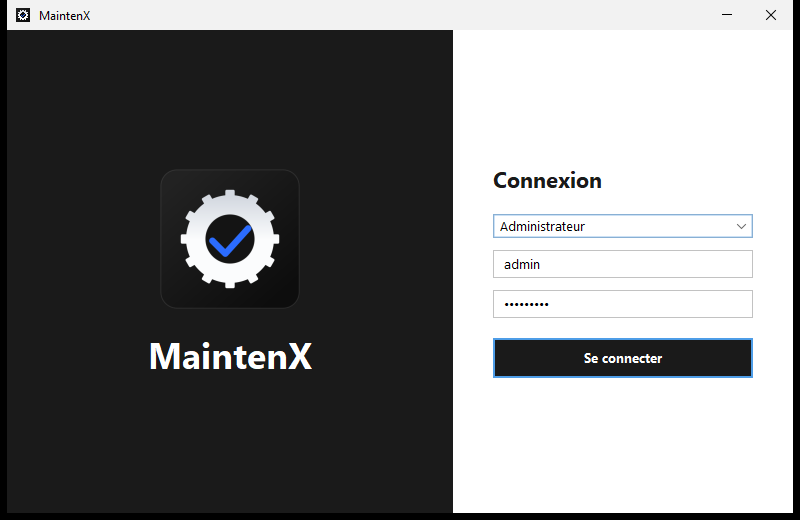
\includegraphics[width=0.784\textwidth]{../images/capture_login.png}
\caption{Écran de connexion}
\end{figure}

L'\textbf{écran de connexion} propose la saisie de l'identifiant et du mot de passe. Les comptes de démonstration sont fournis : administrateur (`admin`/`Admin123!`), responsable (`responsable`/`Resp123!`) et technicien (`tech`/`Tech123!`).
\begin{figure}[htbp]\centering
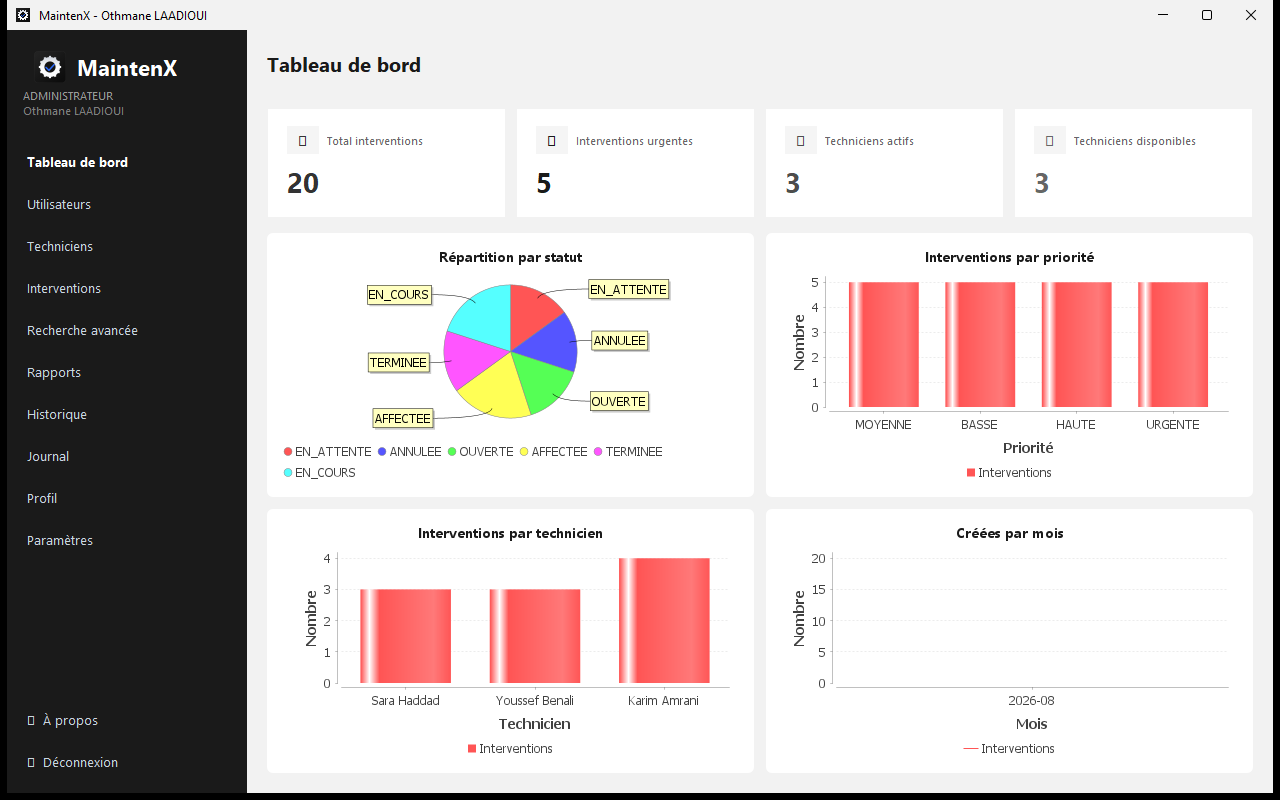
\includegraphics[width=0.878\textwidth]{../images/capture_dashboard.png}
\caption{Tableau de bord principal}
\end{figure}

Le \textbf{tableau de bord} synthétise l'activité : nombre d'interventions par statut, répartition par priorité et indicateurs clés. Il donne au responsable une vision immédiate de l'état du parc.
\begin{figure}[htbp]\centering
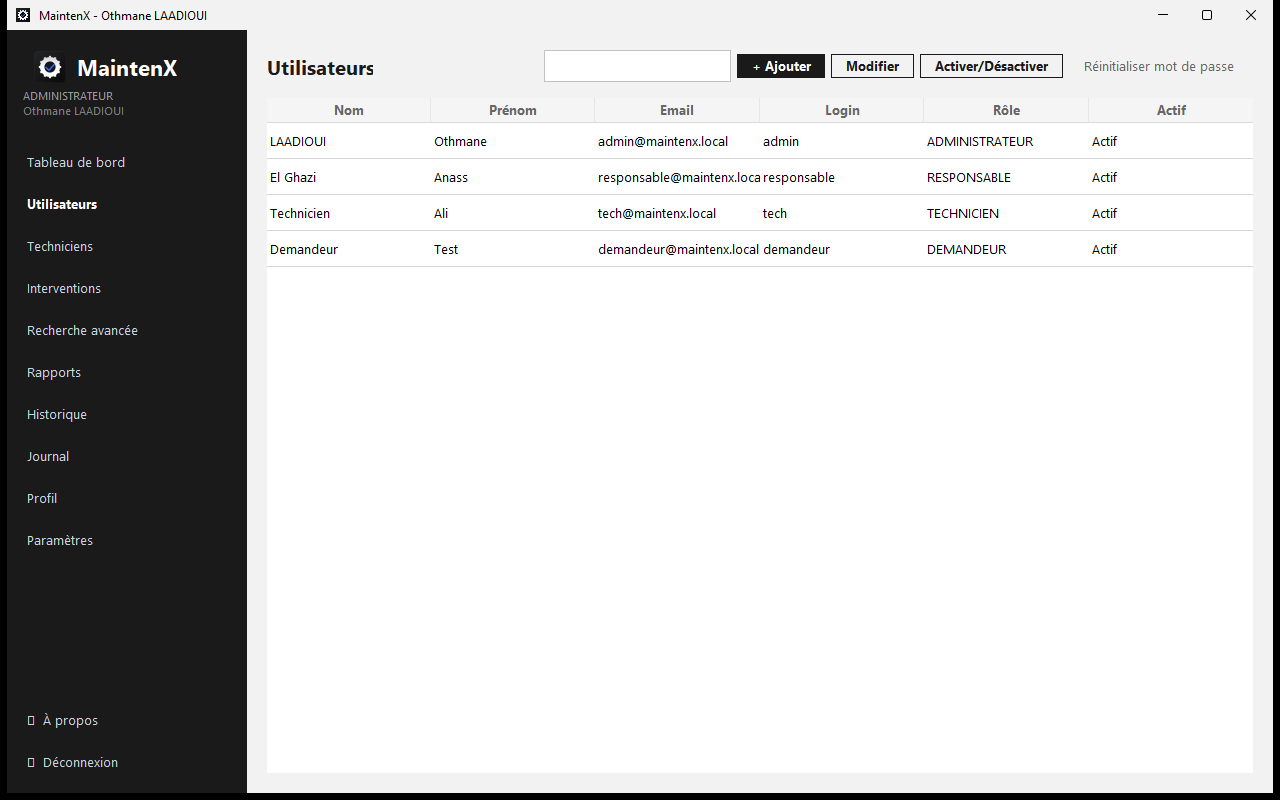
\includegraphics[width=0.878\textwidth]{../images/capture_utilisateurs.png}
\caption{Écran de gestion des utilisateurs}
\end{figure}

La \textbf{gestion des utilisateurs} permet d'ajouter, modifier, activer ou désactiver des comptes et de rechercher un utilisateur par nom, email ou nom d'utilisateur.
\begin{figure}[htbp]\centering
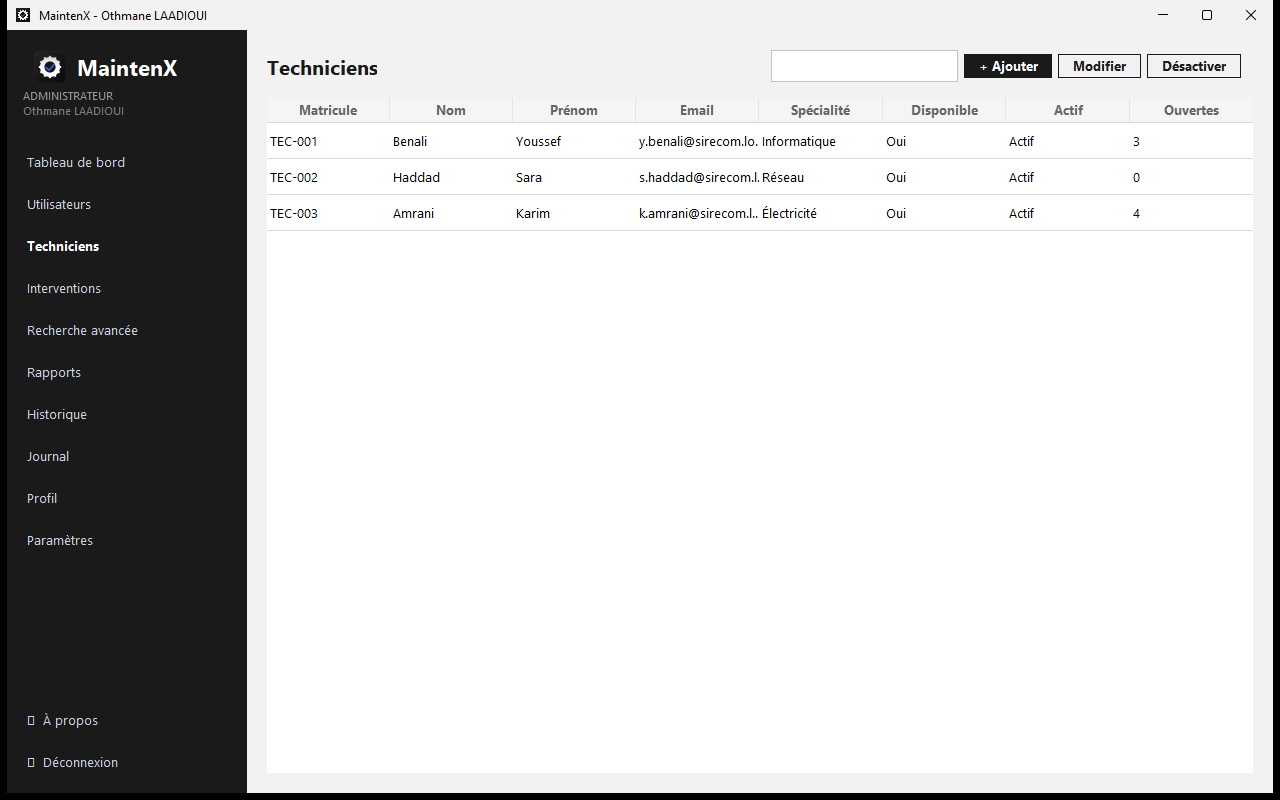
\includegraphics[width=0.878\textwidth]{../images/capture_techniciens.png}
\caption{Écran de gestion des techniciens}
\end{figure}

La \textbf{gestion des techniciens} présente le matricule, la spécialité, la disponibilité et le nombre d'interventions en cours de chaque agent. Seul l'administrateur y a accès.
\begin{figure}[htbp]\centering
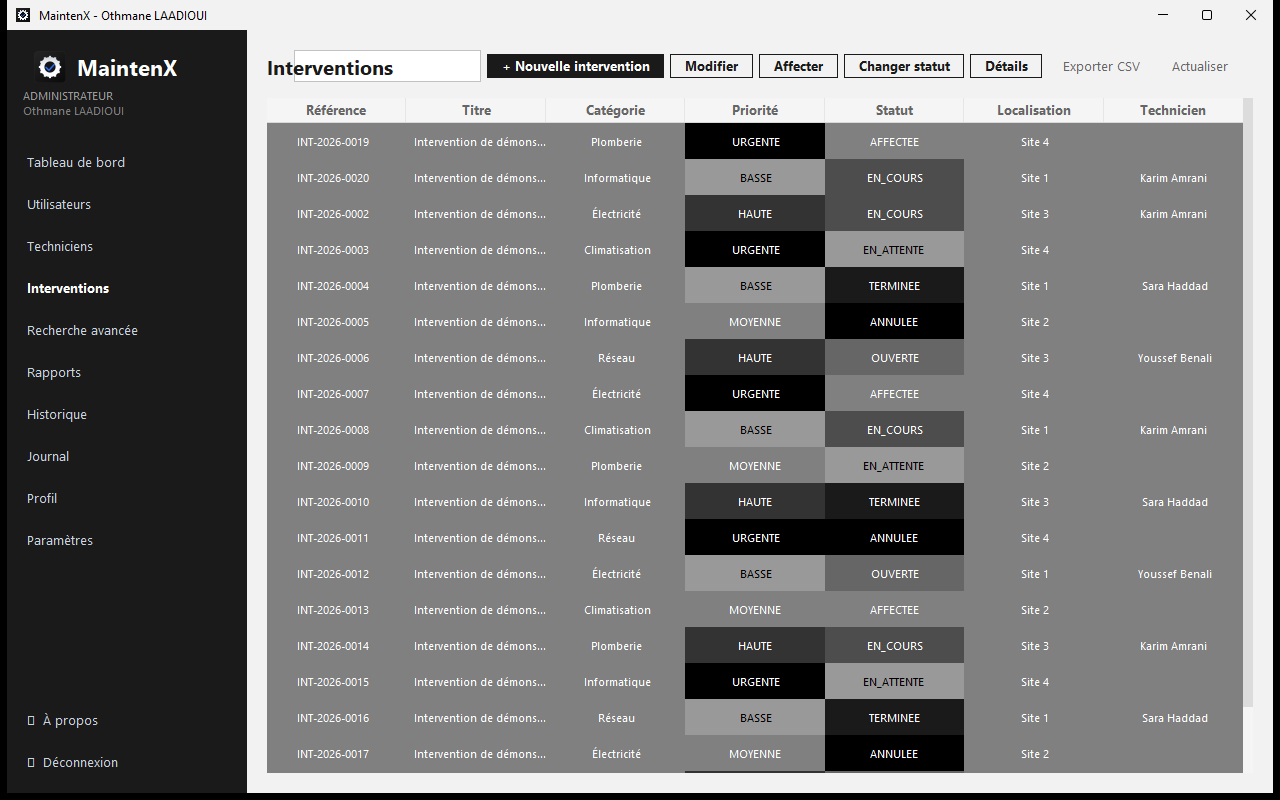
\includegraphics[width=0.878\textwidth]{../images/capture_interventions.png}
\caption{Liste des interventions}
\end{figure}

L'écran des \textbf{interventions} liste les demandes avec leur référence, priorité, statut et coûts. Depuis cet écran, le responsable peut créer, modifier, affecter ou annuler une intervention.
\begin{figure}[htbp]\centering
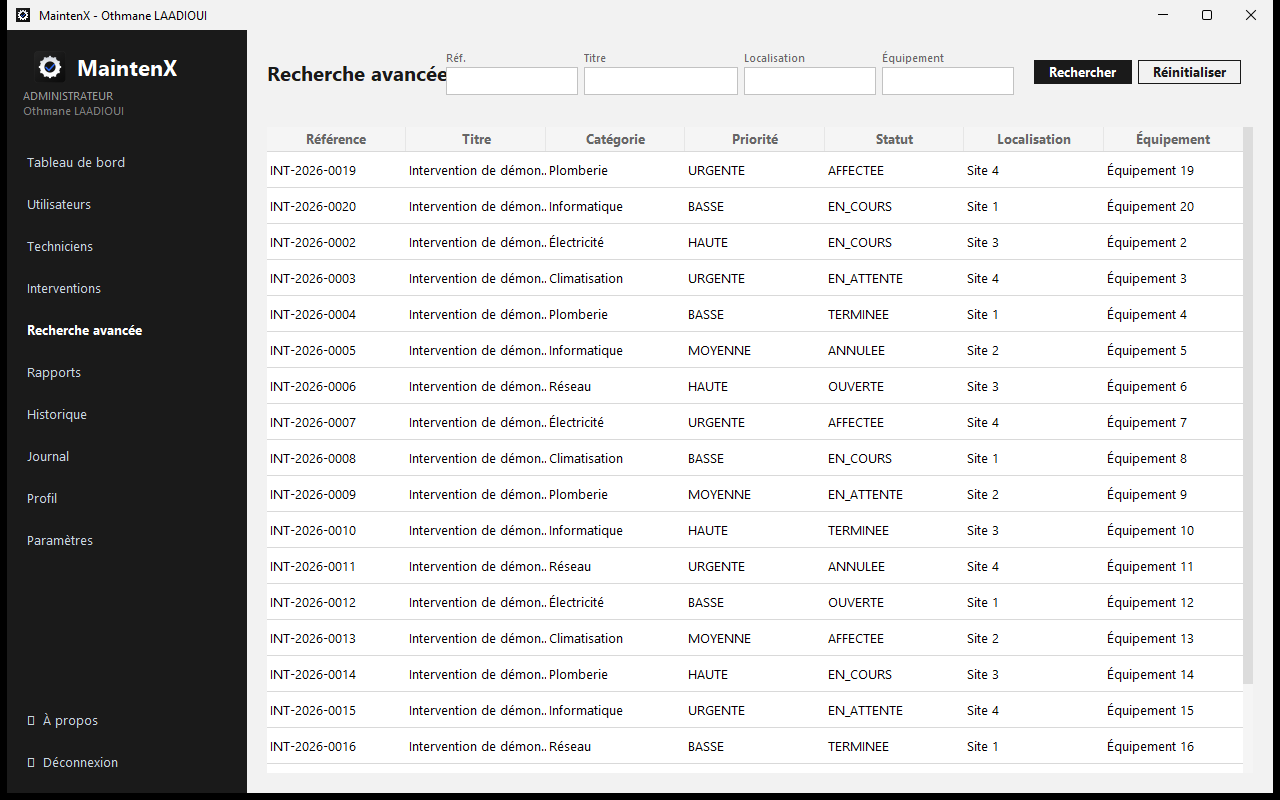
\includegraphics[width=0.878\textwidth]{../images/capture_recherche.png}
\caption{Recherche avancée}
\end{figure}

La \textbf{recherche multicritère} filtre les interventions selon plusieurs critères combinables (référence, statut, priorité, catégorie, localisation, dates, technicien, demandeur).
\begin{figure}[htbp]\centering
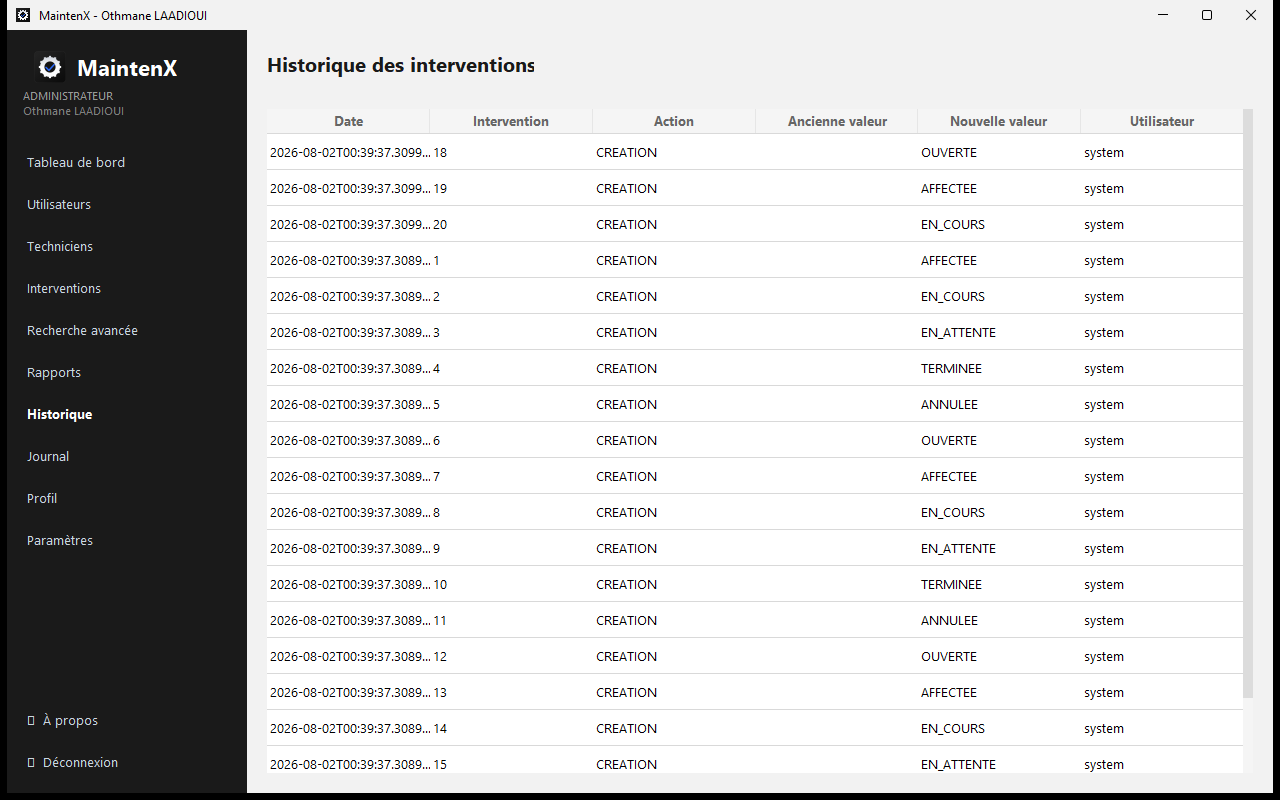
\includegraphics[width=0.878\textwidth]{../images/capture_historique.png}
\caption{Historique d'une intervention}
\end{figure}

L'\textbf{historique} retrace chronologiquement toutes les actions : création, affectation, changement de statut, modification de priorité, clôture… Chaque ligne indique l'acteur, l'ancienne et la nouvelle valeur.
\begin{figure}[htbp]\centering
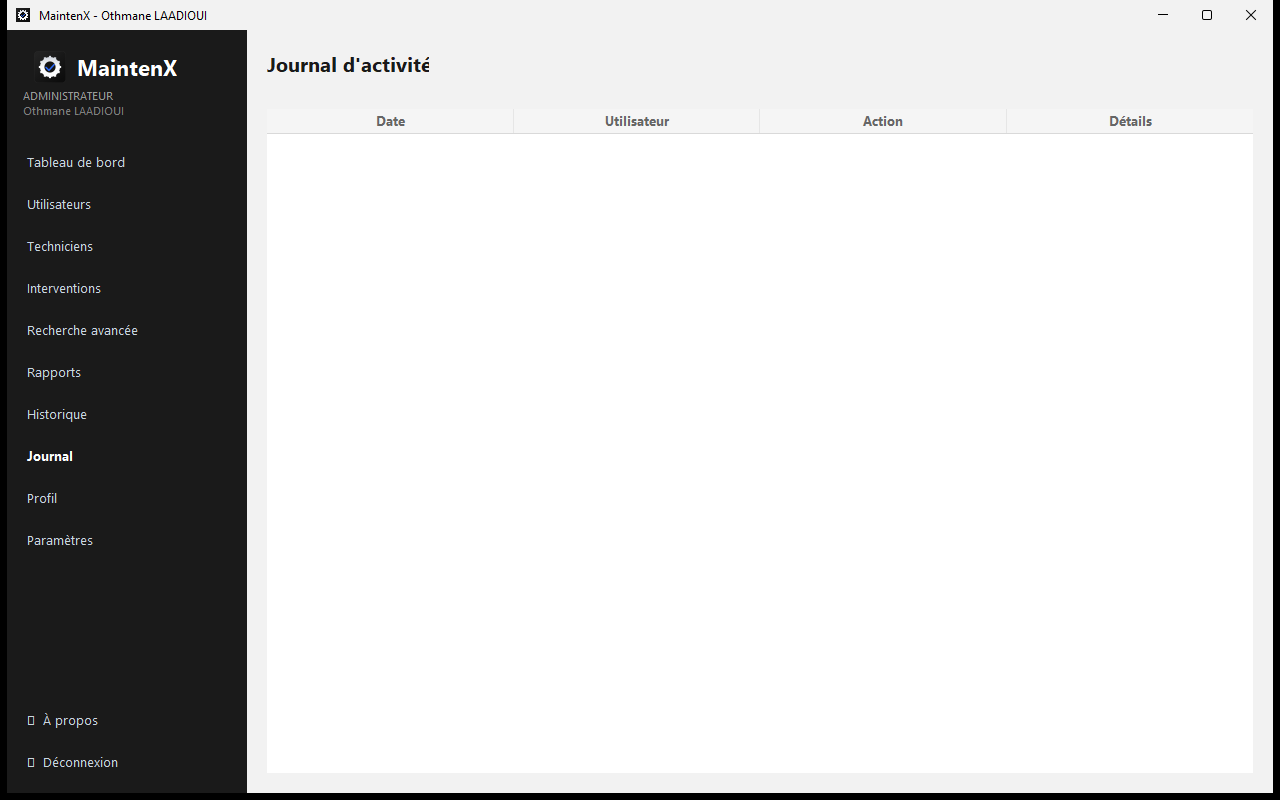
\includegraphics[width=0.878\textwidth]{../images/capture_journal.png}
\caption{Journal d'activité}
\end{figure}

Le \textbf{journal d'activité} est réservé à l'administrateur : il consigne les connexions et les actions globales du système.
\begin{figure}[htbp]\centering
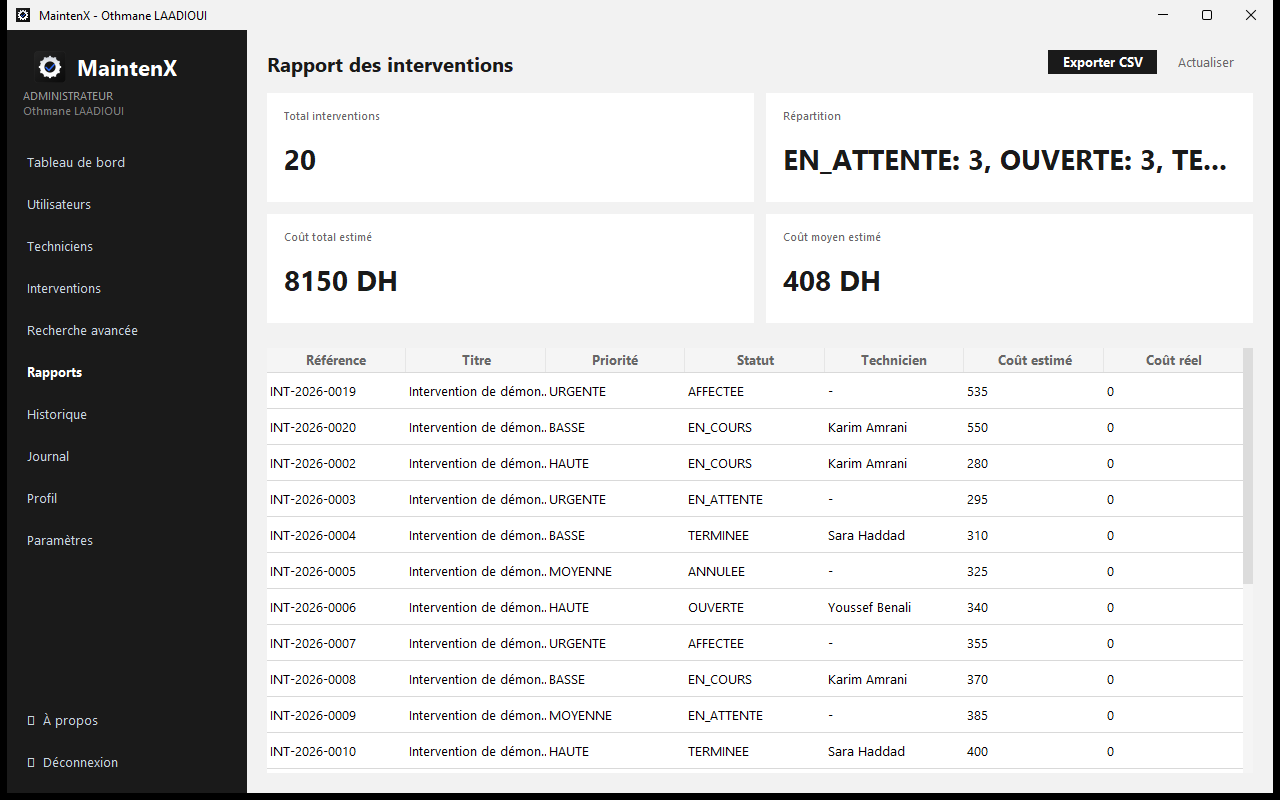
\includegraphics[width=0.878\textwidth]{../images/capture_rapports.png}
\caption{Rapport des interventions}
\end{figure}

L'écran \textbf{Rapport} agrège le total d'interventions, leur répartition par statut, le coût total et le coût moyen estimés, et permet l'\textbf{export CSV}.
\begin{figure}[htbp]\centering
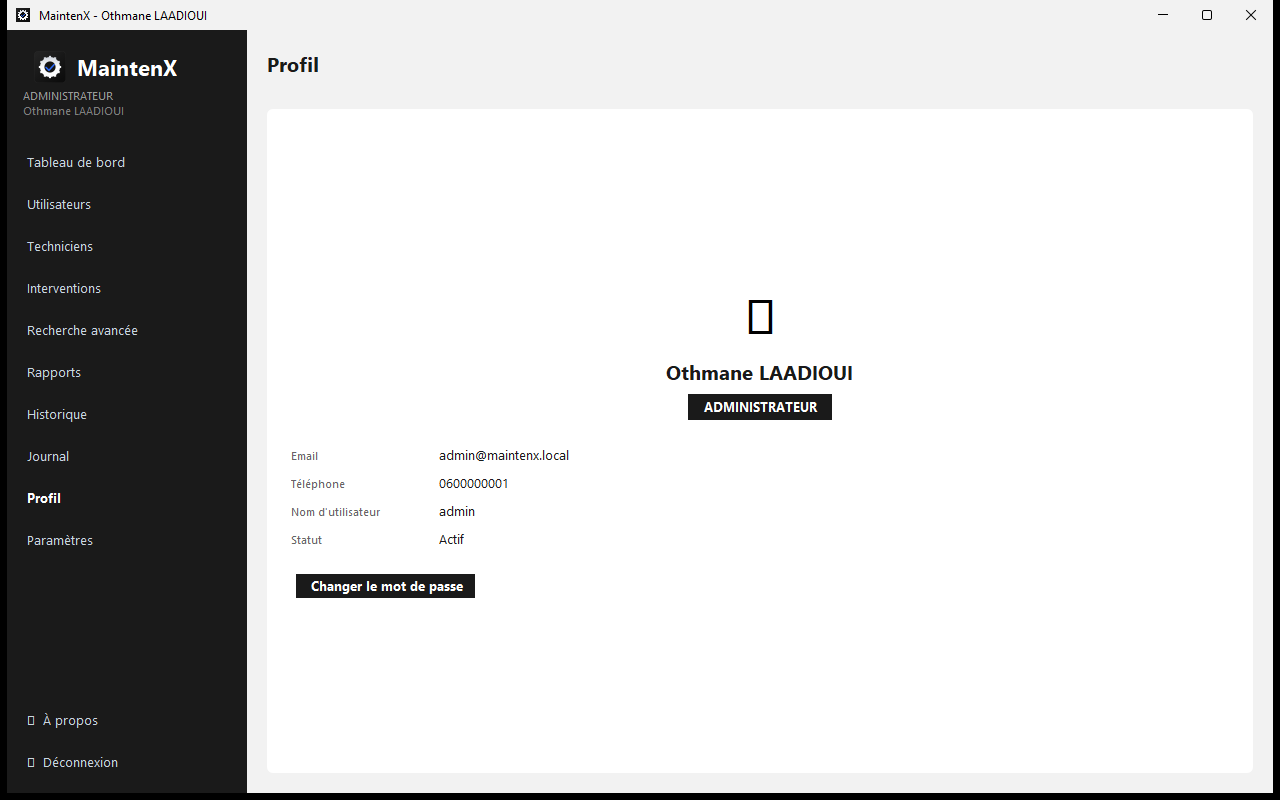
\includegraphics[width=0.784\textwidth]{../images/capture_profil.png}
\caption{Profil utilisateur}
\end{figure}

La page \textbf{Profil} permet à chaque utilisateur de consulter et modifier ses informations personnelles ainsi que son mot de passe.
\begin{figure}[htbp]\centering
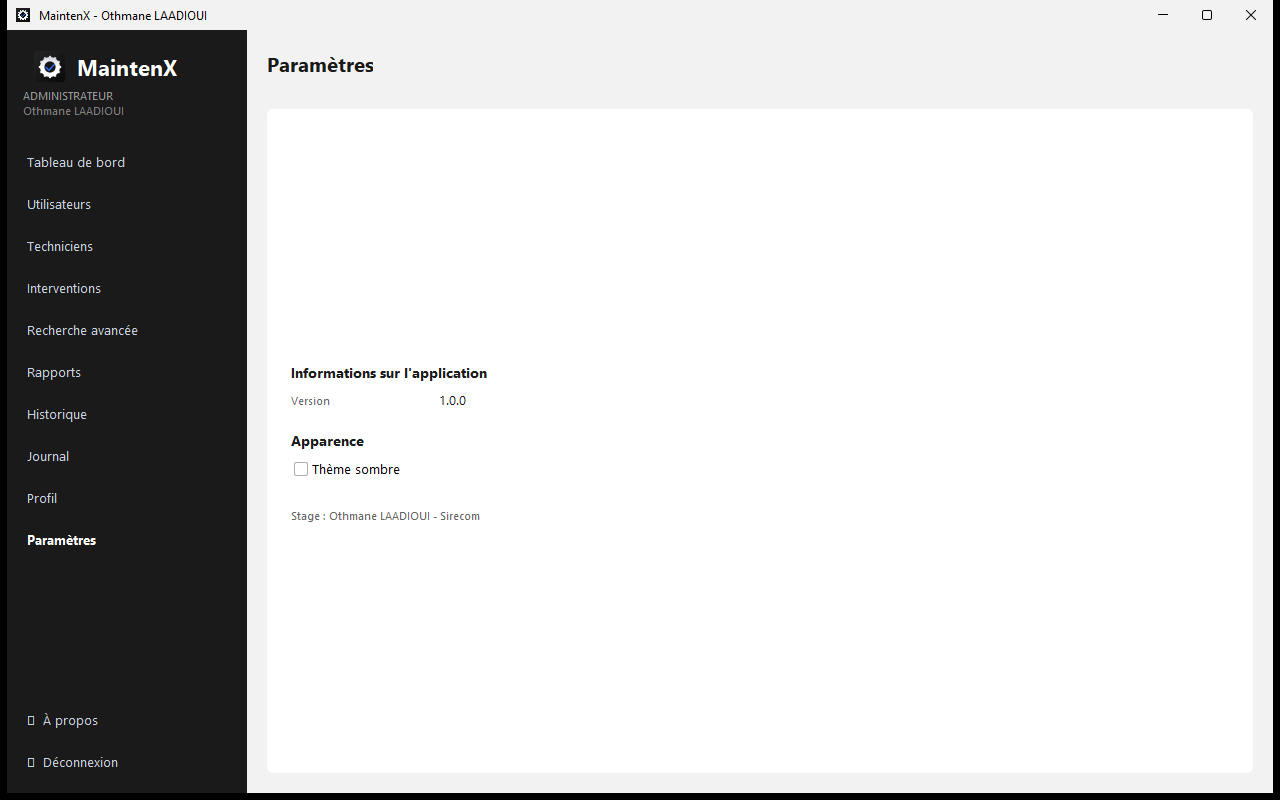
\includegraphics[width=0.784\textwidth]{../images/capture_parametres.png}
\caption{Paramètres de l'application}
\end{figure}

L'écran \textbf{Paramètres} affiche les informations de l'application (version) et permet de basculer entre le thème clair et le thème sombre.
\begin{figure}[htbp]\centering
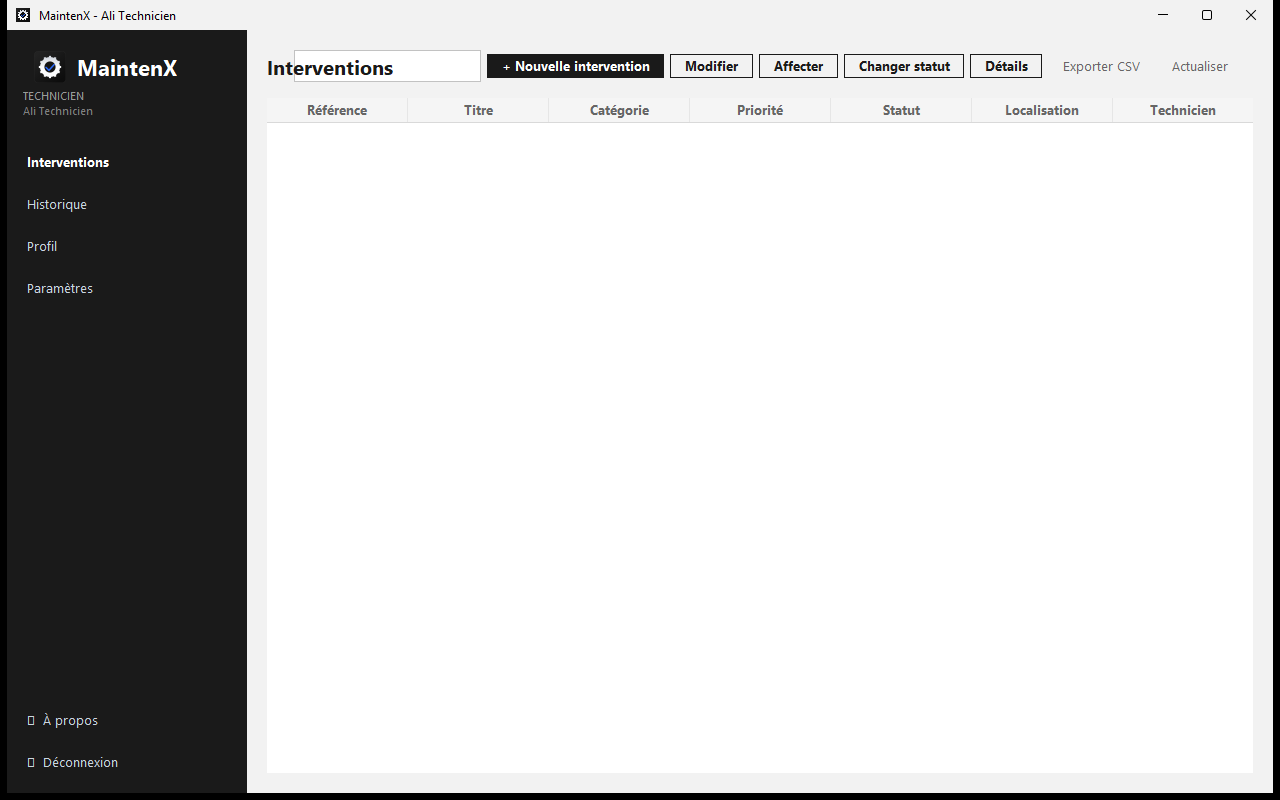
\includegraphics[width=0.878\textwidth]{../images/capture_tech_interventions.png}
\caption{Vue technicien --- interventions affectées}
\end{figure}

Connecté en tant que \textbf{technicien}, l'utilisateur ne voit que ses interventions affectées et dispose d'une navigation réduite (sans les pages de gestion réservées à l'administration), conformément au contrôle d'accès par rôle.
\phantomsection
\subsection*{3.8.1. Parcours de bout en bout}
\addcontentsline{toc}{subsection}{3.8.1. Parcours de bout en bout}

Pour illustrer le fonctionnement réel de l'application, décrivons un scénario complet mettant en jeu les trois rôles.
\begin{enumerate}
  \item \textbf{Étape 1 - Connexion du responsable} : M. Responsable se connecte avec son compte (`responsable`). Le tableau de bord s'affiche avec les statistiques du jour ;
  \item \textbf{Étape 2 - Création de la demande} : il clique sur \guillemotleft{} Interventions \guillemotright{} puis \guillemotleft{} + Nouvelle \guillemotright{}, renseigne le titre, la description, la catégorie (Informatique), la localisation (Site 2) et la priorité (HAUTE). La référence `INT-2026-XXXX` est générée automatiquement et le statut passe à OUVERTE ;
  \item \textbf{Étape 3 - Affectation} : dans la liste, il sélectionne l'intervention et affecte un technicien informaticien disponible. Le statut devient AFFECTEE ;
  \item \textbf{Étape 4 - Traitement par le technicien} : M. Technicien se connecte avec son compte (`tech`), ne voit que ses interventions affectées, démarre l'intervention (EN\_COURS), ajoute son diagnostic puis sa solution, et clôture (TERMINEE) ;
  \item \textbf{Étape 5 - Vérification} : le responsable consulte l'historique de l'intervention : création, affectation, changement de statut, clôture y sont tracés avec horodatage et acteur ;
  \item \textbf{Étape 6 - Contrôle et export} : l'administrateur consulte le journal d'activité global, puis le responsable exporte le rapport au format CSV pour l'archivage.
\end{enumerate}

Ce parcours, répété pendant la phase de tests, confirme que l'application couvre bien l'intégralité du processus métier défini au chapitre 1.
\phantomsection
\chapter*{Chapitre 4 : Tests et déploiement}
\addcontentsline{toc}{chapter}{Chapitre 4 : Tests et déploiement}
\phantomsection
\section*{4.1. Stratégie de test}
\addcontentsline{toc}{section}{4.1. Stratégie de test}

La stratégie de test combine plusieurs niveaux de vérification :
\begin{itemize}
  \item \textbf{Tests unitaires} (JUnit 5) : validation des entrées, règles métier, hachage des mots de passe ; ils s'exécutent sans base de données grâce au magasin en mémoire ;
  \item \textbf{Tests d'intégration} : validation des DAO JDBC contre MySQL (prévus pour l'exploitation réelle) ;
  \item \textbf{Tests fonctionnels manuels} : parcours des écrans avec les comptes des trois rôles, contrôles des transitions de statut et des messages d'erreur ;
  \item \textbf{Tests de non-régression} : chaque correction est suivie de l'exécution complète de la suite (`mvn clean test`).
\end{itemize}
\phantomsection
\section*{4.2. Tests unitaires}
\addcontentsline{toc}{section}{4.2. Tests unitaires}

La suite de tests couvre les classes et règles suivantes :
\begin{table}[htbp]\centering\small
\begin{tabularx}{\textwidth}{|p{3.8cm}|X|}
\hline\rowcolor{hdr}\textbf{Classe de test} & \textbf{Cas vérifiés}\\ \hline
InputValidatorTest & Email valide/invalide, mot de passe trop court, montant négatif, dates non chronologiques, champ vide\\ \hline
PasswordHasherTest & Le condensat ne contient pas le mot de passe, vérification positive\\ \hline
ServiceRulesTest & Création utilisateur, refus des doublons, création d'intervention, affectation, refus d'un technicien inactif, clôture avec solution, refus de clôture sans solution, historique, auto-désactivation de l'administrateur\\ \hline
DaoContractTest & Présence des DAO JDBC pour l'intégration MySQL\\ \hline
\end{tabularx}
\caption{Couverture des tests unitaires}
\end{table}

Exemple de test métier vérifiant le refus de clôture sans solution :
\begin{lstlisting}
@Test
void refusClotureSansSolution() {
    var i = ints.create(intervention(), admin);
    assertThrows(ValidationException.class,
        () -> ints.changeStatus(i.getId(),
                              StatutIntervention.TERMINEE, "", admin));
}
\end{lstlisting}

L'exécution de la suite est intégrée au cycle Maven : `mvn clean test`. Le tableau ci-dessous synthétise les résultats obtenus.
\begin{table}[htbp]\centering\small
\begin{tabularx}{\textwidth}{|p{3.8cm}|X|}
\hline\rowcolor{hdr}\textbf{Critère} & \textbf{Résultat}\\ \hline
Compilation du projet & Réussie (Java 25, Maven 3.9)\\ \hline
Tests unitaires & Tous verts (validations, règles métier, hachage)\\ \hline
Packaging JAR exécutable & Réussi (plugin Shade) - maintenx.jar\\ \hline
Lancement de l'application & Réussi (mode démonstration)\\ \hline
Navigation entre écrans & Corrigée et vérifiée\\ \hline
Connexion aux trois rôles & Vérifiée\\ \hline
\end{tabularx}
\caption{Résultats des tests et de la construction}
\end{table}
\phantomsection
\subsection*{4.2.1. Détail des méthodes de test}
\addcontentsline{toc}{subsection}{4.2.1. Détail des méthodes de test}

La classe `ServiceRulesTest` constitue le cœur de la validation métier. Chaque méthode vérifie un comportement précis :
\begin{table}[htbp]\centering\small
\begin{tabularx}{\textwidth}{|p{3.8cm}|X|}
\hline\rowcolor{hdr}\textbf{Méthode de test} & \textbf{Comportement vérifié}\\ \hline
creationUtilisateurValide & Un utilisateur valide reçoit un identifiant > 0\\ \hline
refusUtilisateurDuplique & Un email déjà utilisé déclenche DuplicateResourceException\\ \hline
creationIntervention & Une intervention créée a le statut OUVERTE et une référence\\ \hline
affectationTechnicien & L'affectation passe le statut à AFFECTEE et renseigne le technicien\\ \hline
refusTechnicienInactif & Affecter un technicien désactivé lève BusinessException\\ \hline
passageTermineAvecSolution & La clôture avec solution positionne TERMINEE et la date de fin\\ \hline
refusClotureSansSolution & Clôturer sans solution lève ValidationException\\ \hline
historiqueCree & Chaque action crée une ligne d'historique\\ \hline
administrateurNeSeDesactivePas & L'administrateur ne peut pas se désactiver lui-même\\ \hline
\end{tabularx}
\caption{Détail des tests métier (ServiceRulesTest)}
\end{table}

Ces tests sont \textbf{déterministes} : ils s'appuient sur le magasin en mémoire et n'exigent ni base de données ni interface graphique, ce qui garantit leur exécution rapide et reproductible dans l'intégration continue.
\phantomsection
\subsection*{4.2.2. Couverture de la validation par couche}
\addcontentsline{toc}{subsection}{4.2.2. Couverture de la validation par couche}

La validation est répartie entre les couches afin de garantir la robustesse à tous les niveaux :
\begin{table}[htbp]\centering\small
\begin{tabularx}{\textwidth}{|X|X|X|}
\hline\rowcolor{hdr}\textbf{Couche} & \textbf{Responsabilité de validation} & \textbf{Exemples}\\ \hline
Présentation & Contrôles légers avant transmission & Champs obligatoires du formulaire\\ \hline
Validation & Validations génériques réutilisables & Email, téléphone, montant $\geq$ 0, dates chronologiques, mot de passe\\ \hline
Service & Règles métier et contrôle des droits & Technicien actif, solution obligatoire, unicité, auto-désactivation\\ \hline
DAO / Base & Contraintes d'intégrité & Clés étrangères, CHECK (cout\_reel $\geq$ 0), UNIQUE, ENUM\\ \hline
\end{tabularx}
\caption{Couverture de la validation par couche}
\end{table}
\phantomsection
\section*{4.3. Tests fonctionnels}
\addcontentsline{toc}{section}{4.3. Tests fonctionnels}

Le plan de tests fonctionnels (disponible dans `docs/tests/`) définit les parcours nominaux et les cas d'erreur attendus. Les principaux cas sont les suivants :
\begin{table}[htbp]\centering\small
\begin{tabularx}{\textwidth}{|X|X|X|}
\hline\rowcolor{hdr}\textbf{Cas} & \textbf{Action} & \textbf{Résultat attendu}\\ \hline
Connexion réussie & Saisir un identifiant/mot de passe valides & Ouverture de la fenêtre principale\\ \hline
Connexion refusée & Saisir un mot de passe erroné & Message d'erreur, accès refusé\\ \hline
Création d'un doublon & Créer un utilisateur avec un email existant & DuplicateResourceException\\ \hline
Affectation d'un technicien actif & Affecter un technicien disponible & Statut passé à AFFECTEE\\ \hline
Affectation d'un technicien inactif & Tenter d'affecter un technicien désactivé & BusinessException\\ \hline
Clôture sans solution & Passer au statut TERMINEE sans solution & ValidationException\\ \hline
Clôture avec solution & Saisir une solution puis clôturer & Statut TERMINEE, date de fin renseignée\\ \hline
Recherche multicritère & Combiner statut et priorité & Liste filtrée correcte\\ \hline
Export CSV & Cliquer sur Exporter CSV & Fichier généré\\ \hline
\end{tabularx}
\caption{Plan de tests fonctionnels (extrait)}
\end{table}
\phantomsection
\subsection*{4.3.1. Procédure de recette}
\addcontentsline{toc}{subsection}{4.3.1. Procédure de recette}

La \textbf{recette} de l'application a été conduite avec les encadrants selon une checklist d'acceptation. Chaque point a été validé à partir de l'interface réelle, avec les trois comptes de démonstration.
\begin{table}[htbp]\centering\small
\begin{tabularx}{\textwidth}{|X|X|X|}
\hline\rowcolor{hdr}\textbf{N°} & \textbf{Critère d'acceptation} & \textbf{Statut}\\ \hline
R01 & Le lancement du JAR ouvre la fenêtre de connexion & Validé\\ \hline
R02 & Les trois rôles se connectent et accèdent aux bons écrans & Validé\\ \hline
R03 & Un mot de passe erroné bloque l'accès avec un message clair & Validé\\ \hline
R04 & Création, modification et désactivation d'un utilisateur & Validé\\ \hline
R05 & Création, modification et désactivation d'un technicien & Validé\\ \hline
R06 & Création d'une intervention avec référence automatique & Validé\\ \hline
R07 & Affectation d'un technicien et refus d'un technicien inactif & Validé\\ \hline
R08 & Suivi des statuts et clôture avec solution obligatoire & Validé\\ \hline
R09 & Recherche multicritère et historique & Validé\\ \hline
R10 & Tableau de bord, rapport et export CSV & Validé\\ \hline
R11 & Journal d'activité réservé à l'administrateur & Validé\\ \hline
R12 & Basculer le thème clair/sombre et le conserver au redémarrage & Validé\\ \hline
\end{tabularx}
\caption{Checklist d'acceptation}
\end{table}

L'ensemble des critères a été validé ; les anomalies constatées en cours de route (notamment l'affichage de la navigation latérale) ont été corrigées puis re-testées.
\phantomsection
\subsection*{4.3.2. Tests d'intégration MySQL}
\addcontentsline{toc}{subsection}{4.3.2. Tests d'intégration MySQL}

Les DAO JDBC ont été conçus pour être testés contre une base MySQL réelle. Le protocole d'intégration est le suivant : création de la base à partir de `database/schema.sql`, chargement des données de démonstration (`sample\_data.sql`), puis exécution de scénarios de CRUD (insertion d'un utilisateur, génération d'une référence d'intervention, recherche multicritère, lecture de l'historique). L'objectif est de valider, en conditions réelles, les requêtes paramétrées et la génération des clés auto-incrémentées. Le test `DaoContractTest` vérifie par ailleurs la présence et l'instanciabilité des DAO JDBC dans le classpath.

Le branchement effectif des services sur ces DAO (au lieu du magasin en mémoire) constitue l'une des perspectives principales, avec pour bénéfice attendu la persistance durable des données de l'entreprise.
\phantomsection
\section*{4.4. Documentation technique}
\addcontentsline{toc}{section}{4.4. Documentation technique}

La documentation technique, livrée dans le dossier `docs/technical/`, comprend :
\begin{itemize}
  \item \textbf{ARCHITECTURE\_MVC\_DAO.md} : description de l'architecture par couches ;
  \item \textbf{DOCUMENTATION\_TECHNIQUE.md} : présentation générale du code et du lancement ;
  \item \textbf{BASE\_DE\_DONNEES.md} : description des tables et des index ;
  \item \textbf{DICTIONNAIRE\_DONNEES.md} : dictionnaire exhaustif des données ;
  \item \textbf{GUIDE\_DEVELOPPEUR.md} : conventions de développement et procédure de contribution ;
  \item \textbf{GUIDE\_DEPLOIEMENT.md} : procédure d'installation et de mise en production.
\end{itemize}
\phantomsection
\subsection*{4.4.1. Gestion des erreurs et journalisation}
\addcontentsline{toc}{subsection}{4.4.1. Gestion des erreurs et journalisation}

La robustesse de l'application repose sur une gestion centralisée des erreurs. Chaque couche lève des \textbf{exceptions métier} typées :
\begin{itemize}
  \item `ValidationException` : saisie non conforme (email, mot de passe, coût négatif, dates…) ;
  \item `BusinessException` : violation d'une règle métier (technicien inactif, auto-désactivation de l'administrateur) ;
  \item `DuplicateResourceException` : unicité violée (email, nom d'utilisateur, matricule) ;
  \item `AuthenticationException` : identifiants invalides ;
  \item `DatabaseException` : défaillance d'accès aux données.
\end{itemize}

La classe utilitaire `ErrorHandler` affiche à l'utilisateur un \textbf{message fonctionnel} (sans trace technique complète) et enregistre les détails dans le fichier de log `logs/maintenx.log`. Cette séparation entre message présenté et trace technique est une exigence de sécurité : elle empêche la fuite d'informations internes vers l'utilisateur final tout en conservant une traçabilité complète pour la maintenance.
\phantomsection
\section*{4.5. Documentation utilisateur}
\addcontentsline{toc}{section}{4.5. Documentation utilisateur}

Le \textbf{Manuel utilisateur} (`docs/user/MANUEL\_UTILISATEUR.md`) explique, de façon illustrée, comment se connecter, naviguer dans l'application, gérer les utilisateurs et les techniciens, créer et suivre une intervention, rechercher, consulter les statistiques et exporter les données. Il est rédigé à destination des trois profils d'utilisateurs.
\phantomsection
\section*{4.6. Déploiement}
\addcontentsline{toc}{section}{4.6. Déploiement}

Le déploiement suit la procédure simplifiée ci-dessous, détaillée dans le guide de déploiement :
\begin{enumerate}
  \item Installer un \textbf{JRE/JDK 25} sur le poste cible ;
  \item Installer \textbf{MySQL 8} et créer la base via le script `database/schema.sql` (tables, contraintes, index, vues) ;
  \item Charger les données de démonstration avec `database/sample\_data.sql` si nécessaire ;
  \item Copier le fichier \textbf{`maintenx.jar`} (JAR exécutable produit par Maven Shade) ;
  \item Configurer la connexion dans `config.properties` (URL JDBC, utilisateur, mot de passe) ;
  \item Lancer l'application : \textbf{`java -jar maintenx.jar`}.
\end{enumerate}

Le packaging par le plugin Shade garantit que toutes les dépendances (FlatLaf, jBCrypt) sont incluses dans un unique JAR portable.
\phantomsection
\section*{4.7. Difficultés rencontrées et solutions}
\addcontentsline{toc}{section}{4.7. Difficultés rencontrées et solutions}
\begin{table}[htbp]\centering\small
\begin{tabularx}{\textwidth}{|p{3.8cm}|X|}
\hline\rowcolor{hdr}\textbf{Difficulté} & \textbf{Solution apportée}\\ \hline
Structurer une application complète sans framework web & Adoption d'une architecture multicouche MVC + Service + DAO stricte, testable et évolutive\\ \hline
Absence de serveur MySQL lors de la soutenance & Mode démonstration en mémoire (DemoDataFactory) activé par défaut, DAO JDBC prêts pour la production\\ \hline
Gestion des dépendances et du packaging & Maven avec plugin Shade produisant un JAR unique exécutable\\ \hline
Sécurisation des mots de passe & Intégration de jBCrypt et exclusion de la configuration du dépôt Git\\ \hline
Cohérence des règles de statut & Centralisation des règles dans les services et tests unitaires dédiés\\ \hline
\end{tabularx}
\caption{Difficultés rencontrées et solutions apportées}
\end{table}
\phantomsection
\chapter*{Conclusion générale et perspectives}
\addcontentsline{toc}{chapter}{Conclusion générale et perspectives}
\phantomsection
\section*{Bilan du projet}
\addcontentsline{toc}{section}{Bilan du projet}

Le projet MaintenX, réalisé au sein de la société SIRECOM, a permis de concevoir et de développer une application de gestion des interventions de maintenance répondant à la problématique posée : la gestion manuelle des demandes ne permettait ni un suivi fiable, ni une priorisation efficace, ni une traçabilité complète. L'application livrée couvre l'ensemble du cycle de vie d'une intervention, de la création à la clôture, en passant par l'affectation des techniciens, le suivi des statuts, l'historisation des actions et la production d'indicateurs.

Sur le plan technique, ce projet a été l'occasion de mettre en pratique les concepts fondamentaux du génie logiciel : analyse des besoins, modélisation UML, architecture multicouche, conception de bases de données relationnelles, programmation Swing, accès aux données avec JDBC et tests automatisés avec JUnit. La séparation stricte entre les couches a permis de produire un code testable et maintenable, et le mode démonstration garantit la présentation du produit en toutes circonstances.

Sur le plan professionnel, ce stage m'a permis de découvrir le fonctionnement d'une entreprise de services, de m'adapter à une équipe et de respecter des délais serrés. Les échanges réguliers avec les encadrants ont également contribué à améliorer la qualité du produit livré.

En regard des objectifs fixés dans l'introduction générale, le bilan est satisfaisant : la quasi-totalité des besoins fonctionnels du cahier des charges a été implémentée et validée, l'architecture multicouche est en place et testée, et l'application est livrée sous une forme exploitable et documentée. Les objectifs de sécurité (hachage BCrypt, messages d'erreur contrôlés) et de traçabilité (historique, journal) ont été atteints.
\phantomsection
\section*{Limites}
\addcontentsline{toc}{section}{Limites}

Le mode par défaut de l'application utilise un magasin de démonstration en mémoire. L'exploitation réelle nécessite d'activer la persistance MySQL : les DAO JDBC sont écrits et prêts, mais leur branchement effectif sur un serveur de production ainsi que la montée en charge restent à valider.
\phantomsection
\section*{Perspectives d'amélioration}
\addcontentsline{toc}{section}{Perspectives d'amélioration}
\begin{itemize}
  \item Brancher directement les services sur les DAO JDBC pour une exploitation MySQL en production ;
  \item Générer des rapports au \textbf{format PDF} en plus du CSV ;
  \item Ajouter une \textbf{notification automatique} (e-mail) lors de l'affectation et de la clôture ;
  \item Introduire une \textbf{pagination} des listes pour de grands volumes de données ;
  \item Développer une \textbf{version web} de l'application ;
  \item Enrichir le tableau de bord avec des \textbf{graphiques temporels} (évolution du nombre d'interventions par mois) ;
  \item Mettre en place un \textbf{système de sauvegarde automatique} de la base de données.
\end{itemize}

Ces perspectives peuvent être organisées en feuille de route : une \textbf{version 1.1} à court terme (persistance MySQL active, rapport PDF, notifications e-mail), puis une \textbf{version 2.0} à moyen terme (version web, pagination, graphiques temporels, sauvegarde automatique). Cette graduation permet d'échelonner les efforts et de livrer de la valeur de façon incrémentale.
\phantomsection
\section*{Compétences acquises}
\addcontentsline{toc}{section}{Compétences acquises}

Ce stage a été l'occasion de consolider et d'enrichir mes compétences :
\begin{itemize}
  \item \textbf{Compétences techniques} : programmation orientée objet en Java, développement d'interfaces Swing, accès aux données avec JDBC, modélisation UML et conception de bases de données MySQL, gestion de projet Maven, écriture de tests unitaires JUnit, versionnement de code ;
  \item \textbf{Compétences méthodologiques} : analyse des besoins, rédaction d'un cahier des charges, conception par couches, suivi d'un planning, documentation technique et utilisateur ;
  \item \textbf{Compétences professionnelles} : communication avec les encadrants, respect des délais, autonomie, esprit d'analyse et de synthèse, capacité à argumenter des choix techniques.
\end{itemize}

En conclusion, MaintenX constitue une base solide et professionnelle qui répond aux objectifs fixés en début de stage et qui peut être étendue progressivement pour accompagner la croissance des besoins de l'entreprise.
\phantomsection
\chapter*{Bibliographie}
\addcontentsline{toc}{chapter}{Bibliographie}
\begin{enumerate}
  \item J. Bloch, \textit{Effective Java}, 3e édition, Addison-Wesley, 2018.
  \item B. Eckel, \textit{Thinking in Java}, 4e édition, Prentice Hall, 2006.
  \item C. S. Horstmann, \textit{Core Java, Volume I - Fundamentals}, 12e édition, Pearson, 2022.
  \item G. Booch, J. Rumbaugh, I. Jacobson, \textit{Le Langage UML : Guide de référence}, Pearson Education.
  \item Y. Khawaja, \textit{Java 21 : Programmer en langage Java}, Eyrolles.
  \item C. Delannoy, \textit{Programmer en Java}, 9e édition, Eyrolles, 2016.
  \item A. Boukerram, \textit{Modélisation UML et bases de données}, Éditions Universitaires.
  \item Oracle, \textit{The Java Tutorials} (traductions et supports de cours EMSI).
\end{enumerate}
\phantomsection
\chapter*{Webographie}
\addcontentsline{toc}{chapter}{Webographie}
\begin{enumerate}
  \item Documentation officielle Java SE : https://docs.oracle.com/javase/
  \item Documentation JDBC : https://docs.oracle.com/javase/tutorial/jdbc/
  \item Documentation MySQL : https://dev.mysql.com/doc/
  \item Documentation Maven : https://maven.apache.org/guides/
  \item Documentation JUnit 5 : https://junit.org/junit5/
  \item Documentation FlatLaf : https://www.formdev.com/flatlaf/
  \item Documentation PlantUML : https://plantuml.com/
  \item Site officiel de la société SIRECOM : documentation interne.
\end{enumerate}
\phantomsection
\chapter*{Annexes}
\addcontentsline{toc}{chapter}{Annexes}
\phantomsection
\section*{Annexe A : Script SQL de création de la base}
\addcontentsline{toc}{section}{Annexe A : Script SQL de création de la base}
\begin{lstlisting}
-- Table utilisateur (extrait)
CREATE TABLE utilisateur (
  id BIGINT PRIMARY KEY AUTO_INCREMENT,
  nom VARCHAR(80) NOT NULL,
  prenom VARCHAR(80) NOT NULL,
  email VARCHAR(160) NOT NULL UNIQUE,
  nom_utilisateur VARCHAR(80) NOT NULL UNIQUE,
  mot_de_passe_hash VARCHAR(255) NOT NULL,
  role ENUM('ADMINISTRATEUR','RESPONSABLE','TECHNICIEN') NOT NULL,
  actif BOOLEAN NOT NULL DEFAULT TRUE,
  date_creation DATETIME NOT NULL DEFAULT CURRENT_TIMESTAMP
) ENGINE=InnoDB DEFAULT CHARSET=utf8mb4;

-- Vue : interventions détaillées
CREATE OR REPLACE VIEW v_interventions_detaillees AS
SELECT i.reference, i.titre, i.statut, i.priorite,
       CONCAT(u.prenom,' ',u.nom) AS demandeur,
       CONCAT(t.prenom,' ',t.nom) AS technicien
FROM intervention i
LEFT JOIN utilisateur u ON u.id = i.demandeur_id
LEFT JOIN technicien t ON t.id = i.technicien_id;
\end{lstlisting}
\phantomsection
\section*{Annexe B : Comptes de démonstration}
\addcontentsline{toc}{section}{Annexe B : Comptes de démonstration}
\begin{table}[htbp]\centering\small
\begin{tabularx}{\textwidth}{|X|X|X|}
\hline\rowcolor{hdr}\textbf{Rôle} & \textbf{Identifiant} & \textbf{Mot de passe}\\ \hline
Administrateur & admin & Admin123!\\ \hline
Responsable & responsable & Resp123!\\ \hline
Technicien & tech & Tech123!\\ \hline
\end{tabularx}
\caption{Comptes de démonstration}
\end{table}
\phantomsection
\section*{Annexe C : Contenu du dépôt du projet}
\addcontentsline{toc}{section}{Annexe C : Contenu du dépôt du projet}
\begin{itemize}
  \item `src/main/java` : code source de l'application ;
  \item `src/test/java` : tests unitaires JUnit 5 ;
  \item `database/` : scripts SQL (schéma, données, vues) ;
  \item `docs/` : documentation technique, utilisateur, tests, rapport ;
  \item `uml/` : diagrammes UML exportés ;
  \item `pom.xml` : configuration Maven.
\end{itemize}
\phantomsection
\section*{Annexe D : Glossaire}
\addcontentsline{toc}{section}{Annexe D : Glossaire}
\begin{table}[htbp]\centering\small
\begin{tabularx}{\textwidth}{|p{3.8cm}|X|}
\hline\rowcolor{hdr}\textbf{Terme} & \textbf{Définition}\\ \hline
Intervention & Demande de maintenance traitée par l'application (création, affectation, suivi, clôture)\\ \hline
Statut & Position d'une intervention dans son cycle de vie (OUVERTE, AFFECTEE, EN\_COURS, EN\_ATTENTE, TERMINEE, ANNULEE)\\ \hline
Priorité & Niveau d'urgence d'une intervention (BASSE, MOYENNE, HAUTE, URGENTE)\\ \hline
Affectation & Désignation du technicien chargé de réaliser une intervention\\ \hline
Diagnostic & Analyse technique de la panne réalisée par le technicien\\ \hline
Solution appliquée & Description de la réparation réalisée (obligatoire pour la clôture)\\ \hline
Référence & Identifiant métier unique d'une intervention, au format INT-AAAA-NNNN\\ \hline
Historique & Trace chronologique des actions réalisées sur une intervention\\ \hline
Journal d'activité & Registre global des connexions et actions du système\\ \hline
Mode démonstration & Fonctionnement sans base de données, à partir d'un jeu de données en mémoire\\ \hline
JAR exécutable & Archive Java autonome, lançable avec la commande java -jar\\ \hline
\end{tabularx}
\caption{Glossaire des termes du projet}
\end{table}
\phantomsection
\section*{Annexe E : Fichier de configuration}
\addcontentsline{toc}{section}{Annexe E : Fichier de configuration}

La connexion à la base de données est centralisée dans `src/main/resources/config.properties`. Ce fichier, ignoré par Git, contient les paramètres sensibles de l'application :
\begin{lstlisting}
# Configuration MaintenX
db.url=jdbc:mysql://localhost:3306/gestion_maintenance
db.user=root
db.password=
app.name=MaintenX
app.version=1.0.0
\end{lstlisting}

La classe utilitaire `ConfigLoader` charge ce fichier au démarrage ; en cas d'absence, un fichier d'exemple (`config.properties.example`) est utilisé pour permettre la compilation sans configuration locale. Cette approche évite de versionner des secrets tout en garantissant le bon fonctionnement du processus de construction.
\phantomsection
\section*{Annexe F : Commandes Maven utiles}
\addcontentsline{toc}{section}{Annexe F : Commandes Maven utiles}
\begin{table}[htbp]\centering\small
\begin{tabularx}{\textwidth}{|p{3.8cm}|X|}
\hline\rowcolor{hdr}\textbf{Commande} & \textbf{Effet}\\ \hline
mvn clean & Supprime les artefacts générés (dossier target/)\\ \hline
mvn compile & Compile les sources\\ \hline
mvn test & Exécute les tests unitaires\\ \hline
mvn package & Construit le JAR (y compris le JAR exécutable via Shade)\\ \hline
java -jar target/maintenx.jar & Lance l'application\\ \hline
\end{tabularx}
\caption{Commandes Maven de construction et de lancement}
\end{table}
\end{document}